\documentclass[aps,epsf,nofootinbib,
notitlepage,showpacs,10pt, unsortedaddress, superscriptaddress]{revtex4-2}

%Loaded above to prevent xcolor clash
\usepackage[svgnames, table]{xcolor}

\usepackage{color}
\usepackage{float}
\usepackage{graphicx}
\usepackage{subcaption}
\usepackage{amsmath}
\usepackage{amsthm}
\usepackage{mathtools}
\newtheorem{theorem}{Theorem}
\theoremstyle{definition}
\newtheorem{example}{Example}[section]
\usepackage{bm}
\usepackage{hyperref}
\usepackage{float}
\usepackage{multirow}
%\usepackage{fancyhdr}
%\fancyfoot[R]{\thepage}
\restylefloat{table}
%\usepackage{nidanfloat}
\usepackage{caption}

\newcommand{\cF}{{\mathcal F}}

% Commands
\newcommand{\braket}[2]{{\left\langle #1 \middle| #2 \right\rangle}}
\newcommand{\bra}[1]{{\left\langle #1 \right|}}
\newcommand{\ket}[1]{{\left| #1 \right\rangle}}
\newcommand{\ketbra}[2]{{\left| #1 \middle\rangle \middle \langle #2 \right|}}
\newcommand{\bfly}[2]{\ket{#1}\!\!\bra{#2}}
%\newcommand{\eq}[1]{Eq.~(\ref{#1})}
%\newcommand{\se}[1]{Sec.~\ref{#1}}
%\newcommand{\avg}[3]{\left<#1|#2|#3\right>}
%\newcommand{\fix}[1]{{\color{red}#1}}
\theoremstyle{definition}
\newtheorem{thm}{Theorem}[section]
\newtheorem{lemma}[thm]{Lemma}


\usepackage{tikz} %to draw graphs
\usetikzlibrary{matrix,positioning}
\usepackage{amsfonts}
\usepackage{amssymb}
\newcommand{\rh}[1]{{\textcolor{blue}{#1}}} %comments by Rebekah
\newcommand{\gs}[1]{{\textcolor{green}{#1}}} %comments by George
\newcommand{\jo}[1]{{\textcolor{red}{#1}}} %comments by Jim
\newcommand{\phil}[1]{{\textcolor{orange}{#1}}} %comments by Phil
\newcommand{\moi}[1]{{\textcolor{magenta}{#1}}}%comments by Moises


\hypersetup{
   colorlinks = true,
    urlcolor=blue
}
\urlstyle{same}
\usepackage[normalem]{ulem}
\usepackage{lipsum}

\newcommand\blfootnote[1]{%
  \begingroup
  \renewcommand\thefootnote{}\footnote{#1}%
  \addtocounter{footnote}{-1}%
  \endgroup
}

\graphicspath{{figures/}}
%%%Tikz%%%
\usepackage{tikz-network}
\usetikzlibrary{fit, shapes.arrows}
\usetikzlibrary{shapes.geometric, arrows}
\usetikzlibrary{positioning,chains,fit,shapes,calc}


\tikzstyle{boxblue} = [rectangle, rounded corners, minimum width=3cm, minimum height=1cm,text centered, draw=black, fill=blue!30]
\tikzstyle{boxred} = [rectangle, rounded corners, minimum width=3cm, minimum height=1cm,text centered, draw=black, fill=red!30]
\tikzstyle{boxgreen} = [rectangle, rounded corners, minimum width=3cm, minimum height=1cm,text centered, draw=black, fill=green!30]
\tikzstyle{io} = [trapezium, trapezium left angle=70, trapezium right angle=110, minimum width=3cm, minimum height=1cm, text centered, draw=black, fill=orange!30]
\tikzstyle{process} = [rectangle, minimum width=3cm, minimum height=1cm, text centered, draw=black, fill=orange!30]
\tikzstyle{decision} = [diamond, minimum width=3cm, minimum height=1cm, text centered, draw=black, fill=green!30]
\tikzstyle{arrow} = [thick,->,>=stealth]

% Define block styles
\tikzstyle{decision} = [diamond, draw, fill=blue!20, 
    text width=4.5em, text badly centered, node distance=3cm, inner sep=0pt]
\tikzstyle{block} = [rectangle, draw, fill=blue!20, 
    text width=5em, text centered, rounded corners, minimum height=4em]
\tikzstyle{line} = [draw, -latex']
\tikzstyle{cloud} = [draw, ellipse,fill=red!20, node distance=3cm,
    minimum height=2em]

%Fix float images
\usepackage{float}

%Neat Tables

\usepackage{array, booktabs, makecell, multirow}


%math packages
\usepackage{amsmath,calc}
%For LP writing
\newlength{\LPlhbox}

%Enumerate renumbering
\newcommand\setItemnumber[1]{\setcounter{enumi}{\numexpr#1-1\relax}}

%Defining a color based on a plot
\definecolor{graphPurple}{RGB}{185,75,185}

%added to display algorithm -moi
%\usepackage{algorithm,algpseudocode}
\usepackage{algorithm}
%\usepackage[chapter]{algorithm}
\usepackage{algpseudocode}

\usepackage[normalem]{ulem}
%\usepackage{pdfpages}
%\usepackage{algpascal}
%\numberthis
\usepackage{subcaption}
\usepackage{caption}
\usepackage{bm}
\algnewcommand{\To}{\textbf{To }}
\algnewcommand\Input{\item[\textbf{Input:}]}%
\algnewcommand\Output{\item[\textbf{Output:}]}%
% no in and out of math mode!
\newcommand{\Fun}[1]{\mathrm{#1}}

\begin{document}

\markboth{First author}
{Graph decomposition techniques for solving CO problems with VQAs}

\title{Graph decomposition techniques for solving combinatorial optimization problems with variational quantum algorithms}

\author{Moises Ponce}
\email{mponce@tennessee.edu}
\affiliation{
	Department of Industrial and Systems Engineering\\ University of Tennessee at Knoxville\\Knoxville, TN 37996}

	
\author{Rebekah Herrman}
%\email{rherrma2@tennessee.edu}
\affiliation{
	Department of Industrial and Systems Engineering\\ University of Tennessee at Knoxville\\Knoxville, TN 37996}
	
	\author{Phillip C. Lotshaw}
%\email{lotshawpc@ornl.gov}
\affiliation{
	Quantum Computational Science Group\\ Oak Ridge National Laboratory\\ Oak Ridge, TN 37830} \thanks{This manuscript has been authored by UT-Battelle, LLC, under Contract No. DE-AC0500OR22725 with the U.S. Department of Energy. The United States Government retains and the publisher, by accepting the article for publication, acknowledges that the United States Government retains a non-exclusive, paid-up, irrevocable, world-wide license to publish or reproduce the published form of this manuscript, or allow others to do so, for the United States Government purposes. The Department of Energy will provide public access to these results of federally sponsored research in accordance with the DOE Public Access Plan.}
\author{Sarah Powers}
%\email{powersss@ornl.gov}
\affiliation{
	Computer Science and Mathematics Division\\ Oak Ridge National Laboratory\\ Oak Ridge, TN 37830}
	

\author{George Siopsis}
%\email{siopsis@tennessee.edu}
\affiliation{
	Department of Physics and Astronomy\\ University of Tennessee at Knoxville\\Knoxville, TN  37996-1200}

	\author{Travis Humble}
%\email{humblets@ornl.gov}
\affiliation{
	Quantum Science Center\\ Oak Ridge National Laboratory\\ Oak Ridge, TN 37830}
 
\author{James Ostrowski}
\email{jostrows@tennessee.edu}\thanks{corresponding author}
\affiliation{
	Department of Industrial and Systems Engineering\\ University of Tennessee at Knoxville\\Knoxville, TN 37996}


\begin{abstract}
    The quantum approximate optimization algorithm (QAOA) has the potential to approximately solve complex combinatorial optimization problems in polynomial time. However, current noisy quantum devices cannot solve large problems due to hardware constraints.  In this work, we develop an algorithm that decomposes the QAOA input problem graph into a smaller problem and solves MaxCut using QAOA on the reduced graph. The algorithm requires a subroutine that can be classical or quantum--in this work, we implement the algorithm twice on each graph. One implementation uses the classical solver Gurobi in the subroutine and the other uses QAOA. 
    We solve these reduced problems with QAOA. On average, the reduced problems require only approximately 1/10 of the number of vertices than the original MaxCut instances. 
    Furthermore, the average approximation ratio of the original MaxCut problems is 0.75, while the approximation ratios of the decomposed graphs are on average of 0.96 for both Gurobi and QAOA. 
    With this decomposition, we are able to measure optimal solutions for ten 100-vertex graphs by running single-layer QAOA circuits on the Quantinuum trapped-ion quantum computer H1-1, sampling each circuit only 500 times. 
    This approach is best suited for sparse, particularly $k$-regular graphs, as $k$-regular graphs on $n$ vertices can be decomposed into a graph with at most $\frac{nk}{k+1}$ vertices in polynomial time. 
    Further reductions can be obtained with a potential trade-off in computational time. 
     While this paper applies the decomposition method to the MaxCut problem, it can be applied to more general classes of combinatorial optimization problems. 
\end{abstract}
%%


\maketitle

\section{Introduction}


Current quantum devices, commonly referred to as noisy intermediate scale quantum (NISQ) devices, are limited by lack of error correction and imperfect gate control, so shallow circuit depth implementations of algorithms are a necessity \cite{Preskill2018NISQ, Alexeev_2021QCSytemsforSCDisc,Bharti_2022}. Despite the limitations in this regime, a great deal of success has been witnessed in utilizing hybrid quantum-classical algorithms. Variational quantum algorithms (VQAs) utilize a quantum computer to perform operations that require real-valued parameters on some initial state. An outer loop optimizes the parameters via classical optimization techniques \cite{McClean_2016TheoryVHybrid,Cerezo_2021VQAs}.%,Sung_2020VQAsOptimizingModels, Peruzzo_2014VQEonQCU}.

The quantum approximate optimization algorithm (QAOA) \cite{Hogg2000QAOA,Farhi2014FQAOA} is a promising candidate for quantum primacy and is universal for computation \cite{FarhiHarrow2016QAOASup, Morales_2020CompUniversalityQAOA,lloyd2018quantum, herrman2022relating}. Since it is a VQA, it requires classical parameter input, and the parameter choice greatly affects the solution output by the algorithm. There are several classical optimization techniques used to find the optimal parameters, such as reinforcement learning, numerical optimization algorithms, and heuristics \cite{wauters2020reinforcement, Zhou_2020QAOAImplementationPerformance,shaydulin2022transfer,lotshaw2021empirical}. Typically, larger problems require deeper circuit depth, which may introduce prohibitive amounts of noise in near-term processors and also complicates parameter optimization \cite{Guerreschi_2019,Willsch_2020,Zhou_2020QAOAImplementationPerformance, Shaydulin_2019MultiStartQAOA,lotshaw2022scaling,lotshaw2022approximate}. QAOA variations have been introduced that incorporate additional classical parameters and perform at least as well as the original algorithm, even strictly better in some cases \cite{herrman2022multi, vijendran2023expressive, wurtz2021classically}. Previous QAOA research indicates that problem structure impacts solution quality and parameter choice \cite{farhi2020quantum, herrman2021impact, shi2022multi, shaydulin2020classical}. %With the popularity of QAOA, there has been a greater focus on implementing the quantum algorithm on useful problems \cite{QAOAIonQC,QAOAChem}. Applications on physical systems require a large number of qubits, a luxury NISQ devices do not have. 
%Though, QAOA is a hybrid quantum algorithm, there still exists some classical component. Interestingly, some large problems QAOA can solve contain a special structure that can be exploited.
%\rh{I think the point of the previous paragraph is to say that classical optimization is important for QAOA, but it is weird that it starts with variational parameters and the last two sentences feel odd, especially with no citations. I would start this paragraph saying classical optimization is important in qaoa, then list why and cite some work. segue into the fact that maybe more classical optimization can be done to improve QAOA results.}

%Classical optimization on large problems can take advantage of particularly `easy' structures and identifying a set of `complicated' constraints. Relaxations and decompositions 
%techniques when implemented properly can return near optimal solutions
%\cite{50yrsofIP}. Many large problems that can be implemented on QAOA can contain a special structure that can exploited  \rh{what is the purpose of the previous paragraph? can it be rolled into the one before it?}


 Classical optimization methods such as dualization and preprocessing have been studied in the context of QAOA, both in terms of initial state preparation and solution quality \cite{herrman2021globally, tate2020bridging}. More closely related to the current work, two recent approaches, QAOA-in-QAOA (denoted $\mathrm{QAOA}^2$) and multilevel quantum local search (ML-QLS) consider iterative approaches to approximately solving large combinatorial problems by solving sequences of subproblems \cite{ushijima2021multilevel,zhou2023qaoa}. %\gs{[``Parallel sequence" sounds like an oxymoron. Can you expand on how their "parallel" is different from our "serial"? Also, by how much do they manage to reduce the number of qubits?]} 
 The solutions to the subgraphs are merged together, and QAOA is used to solve the resulting modified graph. The technique introduced in this paper differs from them because it solves subgraphs of the original MaxCut graph in series. For three-regular graphs, the solved subgraphs are used to create a modified MaxCut graph that has the same objective as the original graph. %\phil{I thought our approach does not necessarily maintain the objective value (hence the error terms in (8))? I think that needs to be clarified (see my comment near (8)) to support the previous sentence that we have "the same objective as the original graph"} 
 It is unclear, however, how other methods used to solve combinatorial optimization (CO) problems in a classical regime can be used to enhance VQAs. 
 
 In this work, we demonstrate that implementing a decomposition technique on a graph and then running QAOA on the resulting simplified, often weighted, graph can output a solution comparable to, and possibly better than, the original algorithm. Furthermore, in many cases, the number of qubits required to solve the decomposed problem is significantly fewer than the number required to solve the original. %\phil{Is there a statement or two we can make about scalability and generality of the graph decomposition technique here - is it polynomial time or something else, does it apply to regular graph maxcut only or is it more general, etc.?} 
 The decomposition algorithm relies on calculating cut sets of graphs, which can be found in polynomial time, and solving integer programs on small instances to create a reweighted graph, which can be done using classical techniques. Furthermore, the decomposition method can be used on general CO problems that can be formulated as graphs. 

The rest of the paper is organized in the following manner: In Section~\ref{sec:background}, we introduce terminology on graphs, QAOA, and combinatorial optimization problems. In Section~\ref{sec:graphdecomp}, we describe our decomposition approach on QUBO problem, outline an algorithmic framework, display case on applying the decomposition technique on a MaxCut instance, and provide an example of the decomposition algorithm iterating on a single graph. We then discuss the effect of decomposition techniques as preprocessing for QAOA in Section~\ref{sec:qaoadecomp}. Finally, we conclude with a discussion in Section~\ref{sec:discussion}. 

%\rh{see a comment here about making underlined text a paragraph, but I don't see underlined text near here}

\section{Background}\label{sec:background}
We now introduce relevant graph theory, QAOA, and CO problem terminology and concepts.
\subsection{ Graph Theory}\label{subsec:graphbackground}

An undirected weighted graph $G=(V,E,J)$ consists of three sets: \textit{vertices}, $V$, \textit{edges}, $E$, and \textit{weights}, $J$. $V$ is a nonempty, typically finite set, while the set $E$ is a collection of unordered pairs in $V \times V$. The $|V| \times |V|$ matrix $J$ encodes the weights of the graph, where $J_{ij}$ contains the weight of edge $(i,j),$ for $i$ not equal to $j$, and $J_{ii}$ contains the weight of vertex $i$. 
%By virtue of a graph being undirected, the pairs in $E$ are unordered i.e. one may traverse a vertex to an edge to another vertex in either direction. 

A graph is said to be \textit{connected} if one can traverse edges of the graph from one vertex to any other vertex in the graph. For a given connected graph, the removal of a set of vertices can disconnect into a number of components. A set of vertices whose removal disconnects a graph is called a \textit{vertex cut set}. For example, it is possible to split the graph in Fig.~\ref{fig:example1} into three disconnected components by removing vertex $1$ and $3$. A \textit{minimum vertex cut set} is the minimum number of vertices whose removal disconnects the graph into at least two nonempty components. The minimum number of vertices needed to disconnect the graph in Fig.~\ref{fig:example1} is one: vertex $3$ disconnects the graph on its own, as does vertex $1$. Let $S \subset V(G)$. The \textit{induced subgraph}, $G[S]$, is a graph that has vertex set $S$ and its edge set  consists of all edges in $G$ that have both endpoints in $S$. %Removing vertex $3$ splits the graph into two nonempty sets. 
%\rh{define regular graph, neighborhoods, etc.}
\begin{figure}
    \centering
    \begin{subfigure}{0.3\textwidth}
        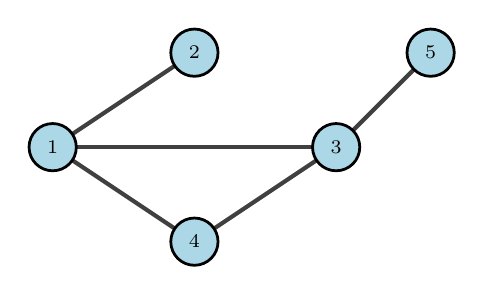
\begin{tikzpicture}[scale = 0.6]
        \Vertex [IdAsLabel, y=1] {1} \Vertex[IdAsLabel,x=3,y=3]{2} \Vertex[IdAsLabel, x=6, y =1]{3} \Vertex[IdAsLabel, x=3,y=-1]{4}
        \Vertex[IdAsLabel, x=8, y = 3]{5} 
        \Edge(1)(2)
        \Edge(1)(3)
        \Edge(1)(4)
        \Edge(4)(3)
        \Edge(3)(5)
        % \draw[red, style=dashed] (0, 0) .. controls (3.5,-4) .. (3.5, 1);
        % \draw[red, style=dashed] (5, 1) .. controls (5,-1) .. (8, -1);
        \end{tikzpicture}
    \end{subfigure}%
    \begin{subfigure}{0.3\textwidth}
        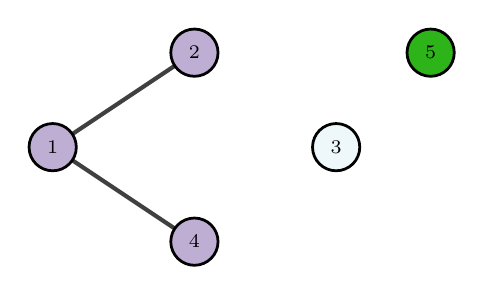
\begin{tikzpicture}[scale = 0.6]
        \Vertex [IdAsLabel, y=1, ,RGB,color={190,174,212}] {1} \Vertex[IdAsLabel,x=3,y=3, ,RGB,color={190,174,212}]{2} \Vertex[IdAsLabel,opacity =.2, x=6, y =1]{3} \Vertex[IdAsLabel, x=3,y=-1,RGB,color={190,174,212}]{4}
        \Vertex[IdAsLabel, x=8, y = 3,RGB,color={45,180,25} ]{5} 
        \Edge(1)(2)
        % \Edge(1)(3)
        \Edge(1)(4)
        % \Edge(4)(3)
        % \Edge(3)(5)
        % \draw[red, style=dashed] (0, 0) .. controls (3.5,-4) .. (3.5, 1);
        % \draw[red, style=dashed] (5, 1) .. controls (5,-1) .. (8, -1);
        \end{tikzpicture}
    \end{subfigure}
    \begin{subfigure}{0.3\textwidth}
        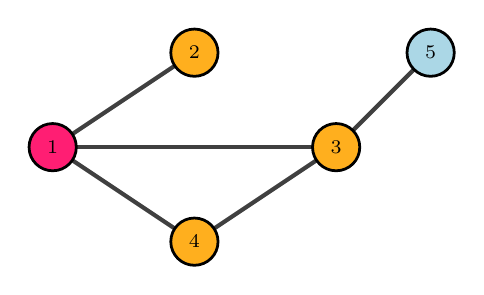
\begin{tikzpicture}[scale = 0.6]
        \Vertex [IdAsLabel, y=1,RGB,color={255,30,115}] {1} \Vertex[IdAsLabel,x=3,y=3,RGB,color={255,175,30}]{2} \Vertex[IdAsLabel, x=6, y =1, ,RGB,color={255,175,30}]{3} \Vertex[IdAsLabel, x=3,y=-1, ,RGB,color={255,175,30}]{4}
        \Vertex[IdAsLabel, x=8, y = 3]{5} 
        \Edge(1)(2)
        \Edge(1)(3)
        \Edge(1)(4)
        \Edge(4)(3)
        \Edge(3)(5)
        % \draw[red, style=dashed] (0, 0) .. controls (3.5,-4) .. (3.5, 1);
        % \draw[red, style=dashed] (5, 1) .. controls (5,-1) .. (8, -1);
        \end{tikzpicture}
    \end{subfigure}
    \caption{Left: An example of a graph. Middle: the minimum cut set $K = \{3\}$ that splits the graph into two nonempty components, purple and green. Right: The neighbors of vertex 1 are colored in orange.}
    \label{fig:example1}
\end{figure}
%As seen in Fig.~\ref{fig:example1}, the creation of the node-node adjacency matrix encodes the graph in matrix form. This matrix will be used as information involving the coupling strength for a two-qubit gate or something.
%The \textit{neighborhood} of a vertex $v$ is the set $N(v) = \{u : e_{u,v} \in E(G)\}$. Each vertex in $N(v)$ is said to be a \textit{neighbor} of $v$. In Fig.~\ref{fig:example1}, $N(1) = \{2,3,4\}$, so all of these vertices are neighbors of $1$.  In a simple, undirected graph, the number of neighbors of a vertex $v$ is called the \textit{degree of v}, denoted $\deg(v)$. The \textit{degree matrix} of $G$, $D_G$, is the diagonal matrix that encodes the degrees of all vertices of $G$.
A graph is said to be $k$-regular if every vertex has $k$ neighbors. Fig.~\ref{fig:example1} is not $k$-regular. 

The aim of the MaxCut problem is to partition the vertex set of a graph into two disjoint sets such that the number of edges with endpoints in each set is maximized. One application of MaxCut is finding the ground states of quantum spin models such as spin glasses \cite{de1995exact, liers2004computing,lotshaw2023simulations}
\subsection{QAOA}\label{subsec:qaoabackground}


QAOA is a classical-quantum hybrid algorithm that requires real-valued parameters input into a parameterized quantum circuit. It requires two unitary operators
\begin{equation*}
U(\beta) = e^{-i \beta H_{B}}
\end{equation*} and
\begin{equation*}
U(\gamma) = e^{-i \gamma H_{C}},
\end{equation*}
\noindent where $H_B$ is called a mixer Hamiltonian, $H_C$ is the cost Hamiltonian that encodes the CO problem being solved, and $\gamma$ and $\beta$ are both real valued numbers between $0$ and $2\pi$.   
 The unitary operators are applied to an initial state $\ket{s}$, which is an eigenstate of $H_B$, in an alternating fashion $p$ times to obtain a final state $\ket{\boldsymbol{\gamma}, \boldsymbol{\beta}}$, %\rh{$\ket{+}^n$ is an eigenstate of $B$ when $B$ is the sum of Pauli-x matrices, so I'm removing $\ket{+}^n$ until we say what $B$ is, and using the commonly used $\ket{s}$ notation here}

\begin{equation*}
\ket{\boldsymbol{\gamma}, \boldsymbol{\beta}} = e^{-i \beta_{p}H_{B}} e^{-i\gamma_{p}H_{C}} \ldots e^{-i \beta_{1}H_{B}} e^{-i\gamma_{1}H_{C}} \ket{s}
\end{equation*}


%The QAOA is described as a discrete version of quantum annealing (QA) \cite{Willsch_2020} or just a trotterized version of QA\cite{Farhi2014FQAOA}. However, a strength in the QAOA is it performs better than QA on difficult graphs with small spectral gaps \cite{Zhou_2020QAOAImplementationPerformance}. Another strength is the QAOA monotonically improves as $p$ increases and is guaranteed to converge as $p$ tends to infinity, however some problem instances can be exactly solved after finitely many iterations.

\noindent This state is then measured to obtain the solution to the CO problem being solved. 

The expected value of the cost Hamiltonian is denoted $\langle H_C \rangle$ and is equal to 
\begin{equation*}
\langle H_C \rangle = \bra{\psi(\boldsymbol{\gamma}, \boldsymbol{\beta})}H_C\ket{\psi(\boldsymbol{\gamma}, \boldsymbol{\beta})}.
\end{equation*}

\noindent The primary metric for success for QAOA is the \textit{approximation ratio}, abbreviated $A.R.$, which is

\begin{equation*}
    A.R. = \frac{\langle H_C\rangle}{C_{max}},
\end{equation*}
\noindent where $C_{max}$ is the optimal solution to the CO problem being solved. The value of $\langle H_C \rangle$ relies on the choice of $\gamma$ and $\beta$, and since the approximation ratio is the primary success metric, $\gamma$ and $\beta$ are chosen to maximize $\langle H_C \rangle$. %  Solving for large problems (i.e. graphs with a large number of vertices) require deep quantum circuit depths. However, finding optimal parameters due to the non-convex and simultaneous optimization of an exponential number of parameters \cite{McClean_2018BarrenPlateaus, Shaydulin_2019MultiStartQAOA, Zhou_2020QAOAImplementationPerformance}. %The classical component is important as the optimizing of the variational parameters creates a more robust model. 

\subsection{Combinatorial optimization problems}\label{subsec:cobackground}

%\rh{generalize this- write generic qubo stuff}

The goal of combinatorial optimization problems is to maximize or minimize some objective function  
\begin{equation*}
C(z) = \sum_{a} C_a(z)
\end{equation*}
\noindent where $z$ is a bit string of length $n$, and each $C_a(z)$ in the sum is referred to as a clause. In order to solve these types of problems with QAOA, the classical clauses $C_a(z)$ must be converted into Hamiltonians. See \cite{hadfield2021representation} for a detailed overview of how Booleans can be mapped into Hamiltonians.

%{\color{red} First describe general QUBO }
% Quadratic unconstrained binary optimization (QUBO) problems are one type of CO problem. In a QUBO, the objective function is a quadratic function over a set of binary variables,

% \begin{equation*}
% C(z) = \sum_{i}\sum_{j} q_{ij}z_iz_j.
% \end{equation*}
% Here, $q_{ij} \in \mathbb{R}$ and $z_i, z_j \in \{0,1\}$ for all $i,j$. For these types of problems, the goal is to find a bitstring $z^*$ that either maximizes or minimizes $C(z)$.

The MaxCut problem \cite{Karp1972} is an NP-complete combinatorial optimization problem that has been the focus of recent QAOA research. % It has been the focus of QAOA research due to the fact that it is easy to encode into a cost Hamiltonian.
%It is defined as the following: given a graph, find a partition of vertices into two sets such that the number of edges that have a vertex in each set is maximized.% In terms of LP, find a partition in which the objective function is the maximum number of edges being cut between the partitioned sets. Vertices can be assigned a value In this case, let's say $\{-1,1\}$. If an edge has a vertex that is $-1$ and the other vertex is $1$, then the edge is cut. 
%Extending Cook's 1971 theorem, Karp defined the problem as NP-complete \cite{Karp1972}. The NP-hardness of the problem motivates the idea that it is unlikely there exists an efficient classical algorithm that can solve it in polynomial time.
%\rh{why is the below listed as a figure and not an equation?}
% \begin{figure}[H]
%\begin{equation}
 %   \max_{c} C = \frac{1}{2} \displaystyle\sum_{ e_{i,j} \in E} (1 - s_i s_j) \label{eq:classyMaxCut}
%\end{equation}
%\noindent Equation~\ref{eq:classyMaxCut} classical formulation of MaxCut where the solution is of the form $s \in \{-1,+ 1 \}^{n}$
% \end{figure}
In order to map the classical MaxCut formulation to a Hamiltonian, we assign a qubit to each $v \in V$. Each clause in the classical formulation is written in terms of an edge of the graph, $e_{i,j}$, and is written as

\begin{equation*}
C_{i,j} =  \frac{1}{2}  ( \mathbb{I} - \sigma_{i}^{z}\sigma_{j}^{z}),
\end{equation*}
\noindent in the Hamiltonian formulation. The total cost Hamiltonian is the sum of clauses
\begin{equation*}
    H_C = \displaystyle\sum_{ e_{i,j} } C_{ i,j }
\end{equation*}
\noindent where $\sigma_{i}^{z}$ refers to the Pauli-z operator acting on qubit $i$, $\mathbb{I}$ is the $2^n$ identity matrix, and $|V| = n$.

There are various classical approximate algorithms for solving the MaxCut problem such as Goemans-Williamson's (GW) algorithm \cite{goemans1995improved}, which is guaranteed to achieve an approximation ratio of $0.879$.
However, QAOA is guaranteed to find the optimal solution as the number of iterations $p \rightarrow \infty$ \cite{Farhi2014FQAOA}. This work will focus on using decomposition techniques to solve the MaxCut problem.
%Shown in \cite{Farhi2014FQAOA}, QAOA is guaranteed an approximation ratio at least 0.6924 on 3-regular graphs, which is better than randomly assigning vertices into sets. A remarkable result considering before the GW algorithm, a worst case scenario guarantee could not be provably better than 0.5. Nowadays, this quantum result may leave many unimpressed. However, this result is guaranteed for QAOA for $p = 1$. It is proven that as $p$ increases, the approximation ratio is guaranteed to monotonically increase.


%A classical computer searches for optimal parameters for $2p$ angles $(\boldsymbol{\gamma}, \boldsymbol{\beta})$. For a given graph $G$ and for each edge $e_{ i,j}$, the $p$ depth initialized for the QAOA generates a subgraph of  edges at most distance $p$ away from $e_{ i,j}$. QAOA generates a list of $|E| = m$ subgraphs. The expectation value for each subgraph is computed independently from each other. One can think of this as: QAOA 'sees' only local structures within an edge $e_{ i,j}$ \cite{Gamarnik2013LocalQ,FixedAngleWurtz,farhi2020quantum}. This is problematic considering that graphs can have similar structures locally are different at a macro-level.

\section{Graph Decomposition on QUBO Problems}\label{sec:graphdecomp}

% \rh{change the script $\mathcal{F}$ in equation (2) to $F_{0}F_{1}$. Write description of $c$ derivation after (3)}
%\rh{general comment for this section- I've always been taught not to label an equation unless you reference it somewhere in the text. do you want me to unlabel equations that we don't ever reference?}
%\rh{should this section be in the background? it doesn't contain new information, does it?}

%\moi{All $x$'s were turned into $z$'s. All $z$ were turned into $C(z)$}

Quadratic unconstrained binary optimization (QUBO) problems are one type of CO problem. In a QUBO, the objective function is a quadratic function over a set of binary variables,

\begin{equation*}
C(z) = \sum_{i} \sum_{j\neq i} J_{ij}z_i z_j  + \sum_{i} J_{ii} z_i. \label{eq:objctive}
\end{equation*}


\noindent For these types of problems, the goal is to find a bitstring $z^*$ that either maximizes or minimizes $C(z)$, that is to find
\begin{align}
C_{max} = \max_{z \in \{0,1\}^n} \sum_{i} \sum_{j\neq i} J_{ij}z_i z_j  + \sum_{i} J_{ii} z_i. \label{eq:qubo}.
\end{align}

%Consider a QUBO of the following form:% \phil{The notation $z$ typically refers to bitstrings in the QAOA literature, and you had it denote a bitstring in an earlier version of this paper, but below I think it refers to a cost value. Why not call this $C^\mathrm{max}$, to stick with the notation you set up in the previous section?  The point of the paper is to guide the reader through what you did, and changing notation makes this unnecessarily confusing. 
%If you really want to stick with $z$, then I think the paper should say "note from now on we denote individual cost values with $z$, as opposed to the generic function $C(x)$ described in the previous section." This will help the reader follow what is going on.}


\noindent %\phil{does this $J$ have any relation to the $J$ defined in II.A?  If so, why does this $J$ depend on the degree matrix as defined in II.A?  If not, why is it represented with the same symbol $J$?} 

Visualize~\eqref{eq:qubo} as a weighted graph, $G = (V,E,J)$, on $n$ nodes, where node $v_i$ has node weight $J_{ii}$ and edge $e_{ij}$  has edge weight $J_{ij}$. Using QAOA to solve the above problem will require, at minimum, $n$ qubits. Furthermore, every iteration of QAOA will require $n$ single qubit gates and $|E|$ two qubit gates \cite{herrman2021lower}. 

Classical optimization techniques can be very effective at solving QUBO instances. If a quantum advantage can be seen in QUBO, it will be on large instances (both in terms of $n$ and $|E|$). Unfortunately, near-term quantum computers do not have the hardware needed to solve these large problems (both in terms of the number of qubits and the fidelity needed to perform $p|E|$-many two qubit gate operations). With that in mind, we attempt to solve a large QUBO by instead solving many smaller QUBOs, each of these requiring far fewer qubits and fewer gates. 


\begin{figure}
    \centering
    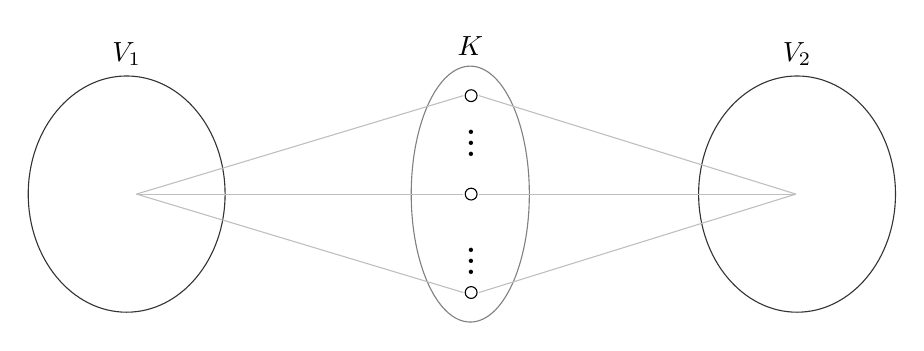
\begin{tikzpicture}[scale=0.5,node distance = 5mm, E/.style = {ellipse, draw=#1, minimum height=3.0cm, minimum width=2.5cm},
    E/.default=black!80!white]
    \node (e1) [E,
                label=above: $V_1$] {};
    % \node (e2) [E,right=of e1,
    %             label=below: ELIPSE TWO] {};
    \node (e3) [E, right=0.0cm and 6cm of e1, label=above: $V_2$] {};
    \node (e2) [E=black!50!white, right=0.0cm and 2.35cm of e1, label=above: $K$, minimum width=1.5cm, minimum height=3.25cm] {};
    \draw (8.75,2.5) circle (0.15cm);
    \draw (8.75,1.5) node [black] {\textbf{\vdots}};
    \draw (8.75,0) circle (0.15cm);
    \draw (8.75,-1.5) node [black] {\textbf{\vdots}};
    \draw (8.75,-2.5) circle (0.15cm);
    \draw[lightgray] (0.25,0) -- (8.55,0);
    \draw[lightgray] (8.95,0) -- (17,0);
    
    \draw[lightgray] (0.25,0) -- (8.55,2.5);
    \draw[lightgray] (8.95,2.5) -- (17,0);
    
    \draw[lightgray] (0.25,0) -- (8.55,-2.5);
    \draw[lightgray] (8.95,-2.5) -- (17,0);
    \end{tikzpicture}
    
    \caption{A graph with cut set $K$ of size $k$ that splits the graph into two components, $V_1$ and $V_2$. }\label{fig:cutsets}
\end{figure}



We can create a {\em restriction} of~\eqref{eq:qubo} by fixing a collection of variables to some values. Let $F_1$ denote the collection of variables fixed to one and $F_0$ the set of variables fixed to zero. The restriction of~\eqref{eq:qubo} with respect to $(F_0, F_1)$ is the following 
\begin{align}
C_{max F_0,F_1} = \max_{z\in \{0,1\}^n|_{F_k}} \sum_i \sum_{j \neq i} J_{ij}z_i z_j  + \sum_i J_{ii} z_i. \label{eq:restrict_qubo}
\end{align}
%\phil{I find this discussion very confusing, as far as I can tell it is switching back and forth between costs and bitstrings, see below.  I recommend stating the cost reformulation separately from the bitstring reformulations, or otherwise clarifying the presentation.}


\noindent Note that we use ${z\in \{0,1\}^n|_{F_k}}$ to denote values for $x$ such that $z_i = 1$ for all $i$ in $F_0$ and $z_i = 1$ for all $i$ in $F_1$.  Note that for any $(F_0, F_1)$, we have that $C_{max F_0, F_1} \leq C_{max}$ %\phil{what does it mean that bitsrings are separated by "$<$", i.e., $z_{F_0, F_1} \leq z$, and why is it relevant? Isn't the relevant thing that the costs associated with these bitstrings are related by an inequality?}. 

Let $K$ be a cut set of $G$ such that its removal leaves two components that have vertex sets $V_1$ and $V_2$ (note that $V_1 \cup V_2 \cup K = V$). For any restriction $(F_0, F_1)$ where $F_0 \cup F_1 = K$, the restricted problem can be written as:
\begin{align}
C_{max F_0, F_1} = \max_{z\in \{0,1\}^n|_{F_k}}   \sum_{l = 1}^2 \big( \sum_{i \in V_l} \sum_{j \in V_l \setminus \{i\}}   J_{ij}z_i z_j  +  \sum_{i \in V_l} \overline{J}_{ii} z_i \big) +    c, \label{eq:decomp}
\end{align}


\noindent where
$\overline{J_{ii}}  = J_{ii} + \sum_{j \in F_1}  J_{ij}$ and 
$c$ is the constant term $\sum_{i \in F_1}\sum_{j \in F_1 \setminus\{i\}} J_{ij}   +  \sum_{i \in F_1} J_{ii}$. When applying a restriction $(F_0, F_1)$. Note that for this restriction, the variables representing vertices in $V_1$ are independent of those in $V_2$, meaning that:

$$C_{max F_0, F_1} = C_{max F_0, F_1}^1 + C_{max F_0, F_1}^2 + c, $$

\noindent %\phil{what does it mean to add the number $c=\sum_{i \in F_1}\sum_{j \in F_1 \setminus\{i\}} J_{ij}   +  \sum_{i \in F_1} J_{ii}$ into a bitstring $z$?} 
where
\begin{align}
C_{max F_0, F_1}^1 = \max_z &      \sum_{i \in V_1} \sum_{j \in V_1\setminus\{i\}}   J_{ij}z_i z_j  +  \sum_{i \in V_1} \overline{J}_{ii} z_i \label{eq:sub1}\\
C_{max F_0, F_1}^2 = \max_z &      \sum_{i \in V_2} \sum_{j \in V_2\setminus\{i\}}   J_{ij}z_i z_j  +  \sum_{i \in V_2} \overline{J}_{ii} z_i. \label{eq:sub2}
\end{align}

Thus, any restriction formed by fixing variables in a cut set can be decomposed into two smaller, independent problems. If one could find the ``correct'' values of the variables  in $K$, those that correspond with the optimal solution, then solving the two subproblems would be equivalent to solving the original problem. In practice, it is unlikely that one would be able to practically (a) find a cut set that decomposes a hard problem into two easy problems and (b) find the correct restriction for that cut set. What is often the case is that one subproblem is very large and difficult while the other subproblem is small and easy. Without loss of generality, we can assume that solving for $C_{max F_0, F_1}^1$ is harder than solving for $C_{max F_0, F_1}^2.$ In order to create a new problem instance that only include the $V_1$ and $K$ variables, and whose optimal solution value is identical to the original QUBO, we compute new coefficients $\hat{J_{ij}}$ and $\hat{J_{ii}}$ for $i,\ j\ \in V_1 \cup K$ and constant $\hat{c}$ such that




\begin{align} C_{max} = \max_{z \in V_1 \cup K} \sum_{i\in V_1 \cup K} \sum_{j\in V_1 \cup K\setminus\{i\}} \hat{J_{ij}}z_i z_j  + \sum_{i\in V_1 \cup K} \hat{J_{ii}} z_i + \hat{c}. 
\label{eq:goal}
\end{align}

\noindent Note that the right hand side contains just variables in $V_1$ and $ K $ while the original problem includes all vertices. We can interpret $\hat{J}$ as the adjacency matrix of a new, smaller, weighted graph. 

We can attempt to find such values by the following. Let $s \in \{0,1\}^{|K|}$ be a bit string representing the values of variables in $K$, and let $C_{max_s}$ be the optimal solution to~\eqref{eq:sub2} and $c$ the constant term from~\ref{eq:decomp} where the variables in $K$ are fixed to the value given in $s$. We attempt to find  $\hat{J_{ij}}$, $\hat{J_{ii}}$, and $\hat{c}$ that satisfy the following system of equations.

\begin{align}\label{eq:soq}
    \sum_{ \{i, j | s[i] = s[j] = 1\} } \hat{J_{ij}} +  \sum_{ \{i | s[i] = 1\} } \hat{J_{ii}} + \hat{c} = C_{max_s}  +c &\  \forall s \in \{0,1\}^{|K|}.
\end{align}


If the above system of equations is not feasible, then we would like to determine values of $\hat{J}$, $\hat{J_{ii}}$, and $\hat{c}$ such that the left hand side of~\eqref{eq:goal} is approximately equal to the right hand side. We can attempt to find such values by introducing error terms to~\eqref{eq:soq} and instead finding solutions to the following system of equations: 

\begin{align} \label{eq:soq_approx}
    \sum_{ \{i, j | s[i] =s[j] = 1\} } \hat{J_{ij}} +  \sum_{ \{i | s[i] = 1\} } \hat{J_{ii}}  + \hat{c} +  e_s= z_s &\  \forall s \in \{0,1\}^{|K|}, 
\end{align}

\noindent where $e_s$ indicates the error associated with the partial solution $s$. %\phil{we need to clarify the meaning of the error $e_s$.  We claim in the introduction and the discussion that we maintain the optimal solution, and if so, then what is the meaning of this error?  Does this mean the "error" has no practical meaning, or it is an error on sub-optimal solutions only, or what? } 
Note that~\eqref{eq:soq_approx} is always feasible (as $e_s = C_{max_s}$ and all other variables equal to zero is a solution). With that in mind, we want to find $\hat{J}$, $\hat{J_{ii}}$, and $\hat{c}$ that minimize the error. Note that one can use any metric to measure the error. Throughout this paper we will minimize the sum of all the error terms with the additional constraint that each $e_s \geq 0$. The lower bound of no error can be achieved for graphs that have minimum cut sets of size at most three. 


\begin{theorem}\label{thm:reweight}
    Let  $G = (V,E,J)$ be a weighted graph with cut set  $K$,  $ |K| \leq 3$. Let $V_1$ and $V_2$ be the vertices in the resulting connected components caused by cut $K$.  The proposed approach generates  a weighted graph $G'(V_1 \cup K, E',w')$ such that $C_{max}$ is the value for the optimal bit string for a MaxCut solution to $G$ if and only if $C_(z)_{G'}$ (the projection of $C(z)$ onto the vertices of $G'$ by deleting entries representing vertices in $V_2$) is an optimal solution to the MaxCut problem on $G'$. 
\end{theorem}

\begin{proof}
It is easy to verify that the systems of equations in \eqref{eq:soq} are full rank and invertible for $|K|\leq 3$, since there are three linearly independent equations with three unknowns, giving a unique solution to the $\hat{J}$ values.
\end{proof}


% \rh{motivate it somehow. 3 gives no error so use eq (7), greater can give error. if $|K|>3$, use eq (8)}

\noindent For $K > 3$, it is possible that $e_s > 0$. %For small problems, the error may not affect the solution provided by~\eqref{eq:soq}. However, substantionally larger problems may see variability in performance. Thus, using~\eqref{eq:soq_approx} adds more security and a higher performance guarantee for larger $K$ values compared to~\eqref{eq:soq}.


\subsection{Algorithm for determining $K$, $\hat{J}$ and $\hat{c}$}
%\rh{this section is not clear}
% Here we describe an algorithmic approach for decomposing large MaxCut problems. This process contains two key components: \textbf{1:} an algorithm decomposes a graph $G$ into a graph $\mathcal{G}$ that has a similar/the same expected value as $G$ and \textbf{2:} a sub-algorithm that computes the redistribution of edge weights and calculates  $c$.
% As shown in~\eqref{eq:sub1} and~\eqref{eq:sub2}, we can treat an instance of the MaxCut problem as two separate subproblems that can be solved. In solving the first subproblem that creates restrictions to find $c$, the second subproblem will be solving for $\hat{J}$ for the decomposed graph.


% Implementing~\eqref{eq:soq} is sufficient for $K \leq 3$. Generally,~\eqref{eq:soq_approx} works for $K>0$ and it mitigates any error, thus utilizing~\eqref{eq:soq_approx} is recommended. The main body of the decomposition algorithm will solve for the decomposed graph. Inside the main algorithm is a subalgoritm that solves both subproblems. The subalgorithm will be used to execute the redistribution of the edge weights and node weights of the graph. The subalgorithm will also capture $c$. 

% Important details to mention is that there must be some method in determining $K$, appropriately changing $J$ to $\hat{J}$, and obtaining $c$ and the decomposed graph.
% Given some random graph, the graph may contain various minimal cut sets. This is not an issue. So long as a cut set leaves two nonempty components, then the decomposition method applies. Choosing any minimum cut set to be $K$ is not a concern in this paper. Note then that the size of the restrictions grows exponentially with the size of the cut set. For practicality, it is recommended then to set an upper bound termination criteria and even a lower bound termination criteria as well for time computation purposes. 
%  \rh{change final $c$ to $\hat{c}$ since that is the notation used in previous section- make sure to get it in the algorithm!}
%We now present an algorithm that decomposes an arbitrary graph $G$ into a reduced, weighted graph $\mathcal{G}$ that has the same objective value as $G$ for the MaxCut problem.  

%First we describe Algorithm~\ref{alg:DecompAlg}, the primary algorithmic process. The first step of the algorithm is to find a minimum cut set $K$ that partitions the vertices of $V\setminus K$ into two nonempty sets, $V_1$ and $V_2$. This set can be found in polynomial time, using algorithms such as the Ford-Fulkerson algorithm \cite{ford1956maximal}. Note that there may be many minimum cut sets, so if the entire algorithm is performed on the same graph twice, there is a possibility that the output will be different.

The formal description of the algorithm is presented in Algorithms~\ref{alg:DecompAlg}-~\ref{alg:weight}. Note that at least one vertex is removed from the graph at each iteration and that the algorithm terminates when either the smallest cut set is greater than some predetermined value or if the resulting graph contains just one vertex. As a result, we know the decomposition algorithm will require at most $|V|$-many iterations. In addition, finding minimum cut sets can be found in polynomial time~\cite{ford1956maximal}. However, solving the MaxCut problem for each of the subproblems is exponential in the size of $V_2$. Note, however, that we can use heuristics to approximate the objective values for these problem instances. 

The input of the Algorithm~\ref{alg:DecompAlg} is a graph (either weighted or unweighted) that contains some cut set $K$ that splits the graph into two components and some $M$, where the algorithm terminates if there are no cut sets of size smaller than $M$. Its output is some weighted graph with strictly fewer vertices than the original graph that has an objective value equal to or bounded above by the optimal objective value of the original graph. MaxCut on the resulting decomposed graph can be solved using fewer qubits than the original problem on a quantum device.
To achieve this end, there is a subroutine Algorithm~\ref{alg:weight} that removes a set of vertices $V_2$. By removing these set of vertices, all possible edges whose endpoints are in $K$ are reweighted and $\hat{c}$ is obtained such that the optimal MaxCut solution of the decomposed graph alongside $\hat{c}$ is bounded above by the optimal solution of the input graph.

\begin{algorithm}[H]%\label{alg:covering}
\caption{Decomposition Algorithm}%\label{alg:DecompAlg}
%\label{alg:covering}
\begin{algorithmic}%\label{alg:covering}
    \Input{$G^{(0)}=(V^{(0)},E^{(0)},J^{(0)})$, M}
    \Function{Decomp}{$G^{(0)}$}
      \State initialize $i \leftarrow 0$ and $c \leftarrow 0$ and $G^{(i)} \leftarrow G^{(0)}$
        \State $K^{(i)} \leftarrow$ minimum cut set of $G^{(i)}$, $V^{(i)}_1$, $V^{(i)}_2 \leftarrow G \backslash K$ \Comment{$|V^{(i)}_1| \geq |V^{(i)}_2|$}
        \State $J^{(i)} \leftarrow$ adjacency matrix of $G$
      \While{$|K^{(i)}|  < M $} \Comment{$M$ is a predetermined parameter}
        % \State $\vec{b} \leftarrow$ using \eqref{eq:soq} using the induced graph $K^{(i)} \cup V^{(i)}_2$ using solver of choice
        \Function{Reweight}{$K^{(i)} \cup V^{(i)}_2$} 
            \State \Return $\hat{J}$, $\hat{c}$
        \EndFunction
        \For{$u \neq v \in K\times K$}
            \If{$uv \in V^{(i)}_1 \cup K^{(i)}$}
                \State $J^{(i+1)}_{uv} \leftarrow J_{uv}^{(i)}$
                \ElsIf{$uv \in K^{(i)} \times K^{(i)}$}
                \State  $J_{uv}^{(i+1)} \leftarrow \hat{J}_{uv}$
            \EndIf
        \EndFor
        \State $V^{i+1} = \{V_{1}^{(i)} \cup K^{(i)} \}$
        \State $E^{(i+1)} = E(V^{(i)}_{1}) \cup E(K^{(i)} \times K^{(i)})$
        % \State $\mathcal{G}^{(i)} = (N^{(i+1)}, E^{(i+1)}, w^{(i+1)})$
        \State $\mathcal{G}^{(i)} = (V^{(i+1)}, E^{(i+1)}, J^{(i+1)})$
        \State $G^{(i+1)} \leftarrow \mathcal{G}^{i}$
        \State $\hat{c^{(i)}} \leftarrow \hat{c}$
        \State increment $i$
      \EndWhile
      \State \Return $\mathcal{G}$, $\hat{c}$
    \EndFunction
    \Output{$\mathcal{G}$, $\hat{c}$}
%\End
\end{algorithmic}\label{alg:DecompAlg}
\end{algorithm}


\begin{algorithm}[H]
  \begin{algorithmic}[1]
    \Input{$G^{(i)}$, $K^{(i)}$, $J^{(i)}$, $J^{(i)}$, $V^{(i)}_1$ $V^{(i)}_2$, $i$}
    \Function{Reweight}{G}
    % \State $K \leftarrow$ minimum cut set of $G$ 
    % \State $V_1$, $V_2 \leftarrow$ two components of $G$ if $K$ is removed; $|V_1| \geq |V_2|$
    \State $H  \leftarrow$ induced graph generated from $K \cup V_2$
    \State Generate an array $S$ that contains all possible $s \in \{0,1\}^{|K|}$ 
    \State initialize $\hat{c} \leftarrow 0$
    \State initialize $\vec{b} \leftarrow \vec{0}$
    % \State initialize $\vec{b\prime} \leftarrow \vec{0}$
    \For{$ind \in range(S)$}
        \State Fix the qubits in $k_l \in K$ to either 0 or 1 with respect to the $l^{\text{th}}$ entry in $S[ind]$
        \State $C_s \leftarrow$MaxCut objective value with fixed qubits in set $K$ 
 
    \State $\vec{b}[ind] = C_s$ 
    \EndFor
    % \State $\vec{b} \leftarrow \vec{b}' - \vec{c^{(i)}}$ \Comment{$\vec{c^{(i)}}$ is a vector that contains just entry of $c^{(i)}$}
   
    \State Solve for~\eqref{eq:soq_approx} to find $\hat{J}$
     \State $\hat{c} \pm \hat{c}^{(i)}$
    % \Comment{Use each entry in $\vec{b}$ as each subsequent value of $z_s$}
      \State \Return {$\hat{J}$, $\hat{c}$}
    \EndFunction
    \Output{$\hat{J}$, $\hat{c}$}
  \end{algorithmic}
  \caption{Reweight Algorithm}
  \label{alg:weight}
\end{algorithm}

% \begin{figure}
%     \centering
%     \begin{tikzpicture}[scale=0.55,node distance = 5mm, E/.style = {ellipse, draw=#1, minimum height=3.75cm, minimum width=2.5cm},
%     E/.default=black!80!white]
%     \node (e1) [E,
%                 label=above: $V_1$] {};
%     % \node (e2) [E,right=of e1,
%     %             label=below: ELIPSE TWO] {};
%     \node (e3) [E, right=0.0cm and 6cm of e1, label=above: $V_2$] {};
%     \node (e2) [E=black!50!white, right=0.0cm and 2.35cm of e1, label=above: $K$, minimum width=1.5cm, minimum height=4cm] {};
%     \draw (8,3) circle (0.15cm);
%     \draw (8,1.5) node [black] {\textbf{\vdots}};
%     \draw (8,0) circle (0.15cm);
%     \draw (8,-1.5) node [black] {\textbf{\vdots}};
%     \draw (8,-3) circle (0.15cm);
%     \draw[lightgray] (0.25,0) -- (7.85,0);
%     \draw[lightgray] (8.15,0) -- (15.15,0);
    
%     \draw[lightgray] (0.25,0) -- (7.85,3);
%     \draw[lightgray] (8.15,3) -- (15.15,0);
    
%     \draw[lightgray] (0.25,0) -- (7.85,-3);
%     \draw[lightgray] (8.15,-3) -- (15.15,0);
%     \end{tikzpicture}
    
%     \caption{A graph with cut set $K$ of size $k$ that splits the graph into two components, $V_1$ and $V_2$. }\label{fig:cutsets}
% \end{figure}



\subsection{Example: Decomposition approach }\label{subsec:graphdecompexample}


% The proposed decomposition techniques may change some elements of the problem. 
% For instance, the MaxCut problem on an  unweighted graph is transformed into a MaxCut problem on a weighted graph. It may even be transformed into a problem that is no longer MaxCut (by having a non-zero value for $J_{ii}$). In this section, we refine the proposed method to address purely quadratic QUBOs, that is, QUBOs where the coeffecients on the  linear terms take the value of zero. We can modify the above approach by fixing all of the $\hat{J_{ii}}$ terms to zero when attempting to find solutions that satisfy the system of equations~\eqref{eq:soq_approx}. Further reduction is made by realizing that the constraints in~\eqref{eq:soq_approx} are replicated, as the equations generated by  $z$ and $z^{-1}$ (defined by $z^{-1} = \bf{1} - z$, where $\bf{1}$ is the vector of ones)  are identical. 

We now give an example of  the decomposition approach applied to a graph, $G = (V,E,J)$, pictured in Fig.~\ref{fig:embedding}. $G$ has a minimum cut set $K = \{2,3,4\}$ whose removal splits the vertices of $G$ into two nonempty sets: $V_1=\{5,6\}$ and $V_2=\{1\}$, such that $|V_1| \geq |V_2|$. Algorithm~\ref{alg:DecompAlg} finds this $K$ and then calls Algorithm~\ref{alg:weight} as a subroutine to remove all vertices in $V_2$, add edges in $K$, and re-weight so the new graph has the same objective value as the original. Algorithm~\ref{alg:DecompAlg} will iterate this process until it reaches a termination criteria.
% The optimal MaxCut solution for this graph cuts all nine edges by placing $K'$ into one set and $V_1 \cup V_2$ into another. 

\begin{figure}
    \centering
    \begin{subfigure}{0.3\textwidth}
            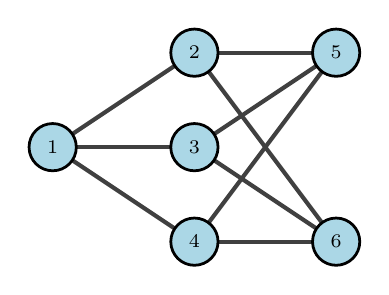
\begin{tikzpicture}[scale = 0.6]
            \Vertex [IdAsLabel, y=1] {1} \Vertex[IdAsLabel,x=3,y=3]{2} \Vertex[IdAsLabel, x=3, y =1]{3} \Vertex[IdAsLabel, x=3,y=-1]{4}
            \Vertex[IdAsLabel, x=6, y = 3]{5} \Vertex[IdAsLabel, x=6, y = -1]{6}
            
            \Edge(1)(2)
            \Edge(1)(3)
            \Edge(1)(4)
            \Edge(4)(6)
            \Edge(4)(5)
            \Edge(3)(6)
            \Edge(3)(5)
            \Edge(2)(6)
            \Edge(2)(5)
            % \draw[red, style=dashed] (0, 0) .. controls (3.5,-4) .. (3.5, 1);
            % \draw[red, style=dashed] (5, 1) .. controls (5,-1) .. (8, -1);
            \end{tikzpicture}
    \end{subfigure}%
    \begin{subfigure}{0.3\textwidth}
            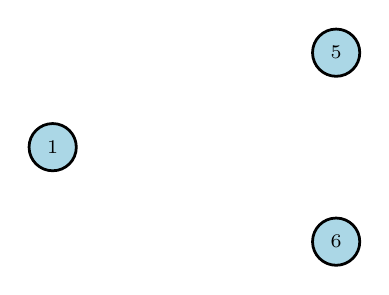
\begin{tikzpicture}[scale = 0.6]
            \Vertex [IdAsLabel, y=1] {1} 
            % \Vertex[IdAsLabel,x=3,y=3]{2} \Vertex[IdAsLabel, x=3, y =1]{3} \Vertex[IdAsLabel, x=3,y=-1]{4}
            \Vertex[IdAsLabel, x=6, y = 3]{5} \Vertex[IdAsLabel, x=6, y = -1]{6}
            
            % \Edge(1)(2)
            % \Edge(1)(3)
            % \Edge(1)(4)
            % \Edge(4)(6)
            % \Edge(4)(5)
            % \Edge(3)(6)
            % \Edge(3)(5)
            % \Edge(2)(6)
            % \Edge(2)(5)
            % \draw[red, style=dashed] (0, 0) .. controls (3.5,-4) .. (3.5, 1);
            % \draw[red, style=dashed] (5, 1) .. controls (5,-1) .. (8, -1);
            \end{tikzpicture}
    \end{subfigure}
    \begin{subfigure}{0.3\textwidth}
             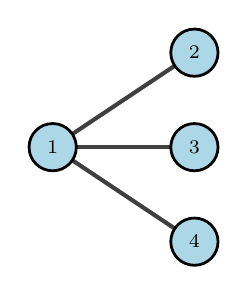
\begin{tikzpicture}[scale = 0.6]
            \Vertex [IdAsLabel, y=1] {1} \Vertex[IdAsLabel,x=3,y=3]{2} \Vertex[IdAsLabel, x=3, y =1]{3} \Vertex[IdAsLabel, x=3,y=-1]{4}
            % \Vertex[IdAsLabel, x=6, y = 3]{5} \Vertex[IdAsLabel, x=6, y = -1]{6}
            
            \Edge(1)(2)
            \Edge(1)(3)
            \Edge(1)(4)
            % \Edge(4)(6)
            % \Edge(4)(5)
            % \Edge(3)(6)
            % \Edge(3)(5)
            % \Edge(2)(6)
            % \Edge(2)(5)
            % \draw[red, style=dashed] (0, 0) .. controls (3.5,-4) .. (3.5, 1);
            % \draw[red, style=dashed] (5, 1) .. controls (5,-1) .. (8, -1);
            \end{tikzpicture}
    \end{subfigure}
    \caption{Left: Graph $G$. Middle: $G$ is split into two components from the removal of $K$. Right:  $V_2 \cup K$}
    \label{fig:embedding}
\end{figure}

% \begin{figure}
%     \centering
%     \begin{tikzpicture}[scale = 0.6]
%     \Vertex [IdAsLabel, y=1] {1} \Vertex[IdAsLabel,x=3,y=3]{2} \Vertex[IdAsLabel, x=3, y =1]{3} \Vertex[IdAsLabel, x=3,y=-1]{4}
%     \Vertex[IdAsLabel, x=6, y = 3]{5} \Vertex[IdAsLabel, x=6, y = -1]{6}
    
%     \Edge(1)(2)
%     \Edge(1)(3)
%     \Edge(1)(4)
%     \Edge(4)(6)
%     \Edge(4)(5)
%     \Edge(3)(6)
%     \Edge(3)(5)
%     \Edge(2)(6)
%     \Edge(2)(5)
%     % \draw[red, style=dashed] (0, 0) .. controls (3.5,-4) .. (3.5, 1);
%     % \draw[red, style=dashed] (5, 1) .. controls (5,-1) .. (8, -1);
%     \end{tikzpicture}
%     \caption{Graph $G$ }\label{fig:embedding}
%     % \rh{you say unweighted but some readers might interpret this as weighted, even though the weights are the same. I would remove edge labels}}
% \end{figure}

Next (Algorithm~\ref{alg:weight}), %\phil{we should explain how Algorithm 1 comes in and how it relates to the algorithm 2 step for this example.} 
we solve the subproblem on the subgraph generated by the vertices in $V_2$ and $K$ for all of the $2^{|K|}$ possible values of vertices in $K$. This is shown in Table~\ref{table:example3sp1solutions}. Using these values, we set up the system of equations as shown in~\eqref{eq:soq} to find the weights of the new edges in $K$. Note that since $|K|$ is three, we know there is an exact  solution to the reweighting problem, so we can solve the system of equations~\eqref{eq:soq} instead of the linear program~\eqref{eq:soq_approx}. %\phil{I think this should be solving for $\hat J_{ij}$, right? The $w$ notation is not what is used in most of the rest of the paper and that makes it confusing here...}


% \moi{Since this is guaranteed to be exact, this is why $c$ is not $\hat{c}$, correct?}
\begin{align}  
 & \hat{c} = 3 & (s = 000)\\
 & \hat{J}_{24} + \hat{J}_{34} + \hat{c}= 2 & (s = 001)\\
 & \hat{J}_{23} + \hat{J}_{34} + \hat{c} = 2 & (s = 010)\\
  & \hat{J}_{23} + \hat{J}_{24} + \hat{c} = 2 & (s = 100)
  \end{align}

\noindent Solving the above system of equations gives us $\{ \hat{J}_{23} = -0.5, \hat{J}_{24} = -0.5, \hat{J}_{34} = -0.5, \hat{c} = 3\}$. We use this to modify the original graph by removing node $A$ and all incident edges and adding an edges $23$, $24$, and $34$ each with weight -0.5. The constant $\hat{c}=3$ is added to the objective function. The new graph is shown in Figure~\ref{fig:exampledecomp}. Note that the optimal solution to the new graph ($x_5 = x_6 = 1$ and $x_2 = x_3 = x_4 =0$) has objective value of 6. That, plus the constant term of 3 gives 9, which is the optimal solution to the original graph. 


\begin{table}
    \centering
    \begin{tabular}{ccccc|c}
        & \multicolumn{3}{c}{\makecell{Partial\\ Assignments}} & & \multicolumn{1}{c}{} \\%
     \arrayrulecolor{Gainsboro} \cmidrule[\heavyrulewidth](l){2-4}\cmidrule[\heavyrulewidth]{6-6} \arrayrulecolor{black}
        & \makecell{\; $V_2$ \;}&\makecell{\; $V_3$ \;} & \makecell{\; $V_4$ \;} & & \makecell{Subproblem\\Solution} \\
    \midrule
        & 0 & 0 & 0 &  & 3.0 \\
        & 0 & 0 & 1 &  & 2.0 \\
        & 0 & 1 & 0 &  & 2.0 \\
        & 1 & 0 & 0 &  & 2.0 \\
        \bottomrule
    \end{tabular}
        \begin{tabular}{ccccc|c}
        & \multicolumn{3}{c}{\makecell{Partial\\ Assignments}} & & \multicolumn{1}{c}{} \\%
     \arrayrulecolor{Gainsboro} \cmidrule[\heavyrulewidth](l){2-4}\cmidrule[\heavyrulewidth]{6-6} \arrayrulecolor{black}
        & \makecell{\; $V_2$ \;}&\makecell{\; $V_3$ \;} & \makecell{\; $V_4$ \;} & & \makecell{Subproblem\\Solution} \\
    \midrule
        & 0 & 1 & 1 &  & 2.0 \\
        & 1 & 1 & 0 &  & 2.0 \\
        & 1 & 0 & 1 &  & 2.0 \\
        & 1 & 1 & 1 &  & 3.0 \\
        \bottomrule
    \end{tabular}
    \caption{All MaxCut partial assignment subproblem solutions for 3-cut example.}
    \label{table:example3sp1solutions}
\end{table}


\begin{figure}
    \centering
    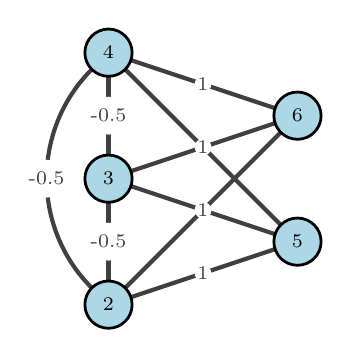
\begin{tikzpicture}[scale = 0.8]
    \Vertex[IdAsLabel,x=3,y=-1]{2} \Vertex[IdAsLabel, x=3, y =1]{3} \Vertex[IdAsLabel, x=3,y=3]{4}
    \Vertex[IdAsLabel, x=6, y = 0]{5} \Vertex[IdAsLabel, x=6, y =2]{6}
    \Edge[label=1](4)(6)
    \Edge[label=1](4)(5)
    \Edge[label=1](3)(6)
    \Edge[label=1](3)(5)
    \Edge[label=1](2)(6)
    \Edge[label=1](2)(5)
    \Edge[bend=-45, label = -0.5](4)(2)
    \Edge[label = -0.5](4)(3)
    \Edge[label = -0.5](3)(2)
    % \draw[red, style=dashed] (0, 0) .. controls (3.5,-4) .. (3.5, 1);
    % \draw[red, style=dashed] (5, 1) .. controls (5,-1) .. (8, -1);
    \end{tikzpicture}
    \caption{Graph $\mathcal{G}$ for 3-Cut Example }
    \label{fig:exampledecomp}
\end{figure}

% \noindent
%The MaxCut solution to $\mathcal{G}'$ is $6$. The parameter $c=3$ is then added to the objective value of $\mathcal{G}'$. This sum gives the original objective value to the original graph i.e. $9$. Thus, the exact MaxCut objective value for $G$ and $\mathcal{G}$ are the identical in value.

%\moi{Should we include here the QAOA objective value on $G'$ vs $\mathcal{G}'$? I ask this to show that there is a slight improvement in QAOA's performance, but this motivates applying the decomposition more iterations}

% \subsection{Example: Algorithm~\ref{alg:DecompAlg}}
% \rh{this section is not clear}
% \moi{I agree. I wrote this section to help motivate why applying more iterations of the decompositions can be helpful. For a 3-regular graph, we only see a decrease of one qubit per iteration most of the time. Also, if we agree that is what we want to focus on here Fig.~\ref{fig:qaoadecomp_iterations} should be moved here to show the improved performance?}
% The prior example demonstrates the decomposition algorithm after one iteration. However, one can decrease the number of qubits needed to solve the MaxCut problem on a given graph by applying multiple iterations of the decomposition algorithm.
% In this example, we are able to construct a smaller graph with a nearly equivalent solution value, up to error.% We have that for MaxCut, any cut set with three or fewer vertices can be used to create a smaller graph with zero error. 

% Conceptually, the decomposition technique decreases the number of vertices in the decomposed graph while monotonically increasing the number of edges in the graph (edges may not increase if $K$ is a clique of size $k$) \rh{is this true? imagine a graph with two cliques of size 10, and two extra vertices, where those two extra vertices are connected to random edges in each of the cliques, and the cliques are not connected to each other (so the two vertices are a cut set). we are removing at least 45 edges when we eliminate $V_1$ and only adding at most 1 edge?}.

 % \gs{But more generally, I have a hard time following the proposed procedure/iteration. It may just be my lack of understanding, but this looks like some kind of a greedy algorithm combined with QAOA. Am I correct to conclude that the reduction in the number of qubits is due to replacing part of the quantum algorithm with a classical algorithm? What happens when $K=G$?} 
 
% Fig.~\ref{fig:graphAtIter0&33} is an example of one of the random 3-regular 100-vertex graphs on which MaxCut is solved in this study. The decomposition algorithm iterates until the termination criteria is met. Let the superscript $^{(t)}$ denote the iteration number, where $^{(0)}$ represents the original graph. Let graph $G^{(0)}$ have a cut set $K^{(0)}$ that partitions the graph into two non-empty vertex sets: $V^{(0)}_1$ and $V^{(0)}_2$. Using the decomposition algorithm, by \eqref{eq:soq}, without loss of generality, $V^{(0)}_2$ is removed from the graph, so the number of vertices is reduced by $|V^{(0)}_2|$. In this example, since the graph is $3$-regular, $|K^{(t)}|=3$ for small $t$. Furthermore, since $G$ is 3-regular, the algorithm will search for cut sets of size three and use these to reduce the graphs before moving on to cut sets of size four. However, the caveat is that since the minimum cut set size is three for the first iterations, any cut set of size three can be chosen in any order. This can lead to cases where edges receive a weight of zero (so the edge is removed from the graph), or where cut sets of size two are created, causing the algorithm to terminate. % It may be that the combination of selecting cut sets that neighbor each other to utilize for \eqref{eq:soq} and the reweigting \eqref{eq:soq_approx} giving an edge of weight zero (i.e. no edge) there are instances where the vertices it chooses leads to the creation of a cut set of size 2, and so the algorithm terminates. 





\section{Implementation and Results}\label{sec:qaoadecomp}

%\rh{are you using QAOA and Gurobi in algorithm 2, when you reweight?}
%\moi{Good question. I was unsure how to solve an LP using QAOA. So, when I solved for the first subproblem, where we solve all $2^{|K|}$ restrictions for $K \cup V_2$, I used QAOA and Gurobi. I could at least do that. However, I did not know how to use QAOA to solve \eqref{eq:soq_approx} so that job went strictly to Gurobi. Meaning, Algorithm~\ref{alg:weight} either used Gurobi-Gurobi or QAOA-Gurobi (SP1-SP2)}\rh{where are SP1 and SP2 defined? are these eq 3 and eq 5?}
%\moi{Well, I believe it is defined at \eqref{eq:sub1} and \eqref{eq:sub2}. The first equation deals with $V_1 \cup K$ and the second equation deals with $V_2 \cup K$ }

We apply the above decomposition algorithm to twenty-five 3-regular 100-vertex MaxCut instances. 

\subsection{Algorithm implementation details}

In order to implement Algorithm~\ref{alg:DecompAlg}, we use max-flow implementation~\cite{networkX,esfahanian2013connectivity} to find a minimum cut set, $K$, of each input graph. The two sets into which the graph is partitioned when the cut set is removed are called $V_1$ and $V_2$, where without loss of generality, $|V_1| \geq |V_2|$. Algorithm~\ref{alg:DecompAlg} then calls on Algorithm~\ref{alg:weight}. In Algorithm~\ref{alg:weight}, each vertex in $K$ is assigned a value $0$ and $1$, and the MaxCut objective for $V_2 \cup K$ is calculated. We test two different approaches to solving these subproblems. The purely classical approach uses Gurobi\cite{gurobi}, a state-of-the art commercial software. We also test using QAOA to find solutions %\phil{I don't understand what this means. You are using QAOA within Alg. 1 to do the decomposition? If so, doesn't this require generating bitstrings, optimizing parameters, etc., and how is that done?  If not, then what do you mean by also testing QAOA to find solutions? }.
 %\moi{Correct. We use QAOA to solve the MaxCut problem for the subgraph $K \cup V_2$. We are fixing the qubits of $K$ to $2^{|K|}$ possible restrictions. Usually, $|V_2|$ for our regular graph tests are about one vertex. So, we are applying QAOA on this subgraph typically only $|K|+1$ many vertices $2^{|K|}$ times} \phil{Okay, it sounds like QAOA is used within algorithm 1 to do the decomposition.  But this needs to be explained. Are you taking samples from QAOA, or expected cost values, or something else? Are you doing multiple parameter optimizations or one?  etc.}
 We note that Gurobi returns an exact optimal solution while QAOA returns a heuristic solution based on the expected cost value, as we now describe. 

The expected value of general Ising problems was derived by Ozaeta, van Dam, and McMahon \cite{Ozaeta_2022}. These formulas, found in Appendix~\ref{app:formula}, were used to calculate the expected value of the subproblem when solved with QAOA \cite{Ozaeta_2022}. The optimal parameters were selected by maximizing the sum of the expected value terms for each problem using the Broyden-Fletcher-Goldfarb-Shanno (BFGS) algorithm \cite{wright1999numerical}. As BFGS terminates in a local minimum, we repeated each optimization 100 times using different random starting parameters.% \moi{The initial values are randomly chosen by $2\pi*$ some uniform distribution value between 0 and 1 that is subtracted by 0.5)}. 
% \phil{does this mean that 100 separate runs each look for optimal parameters and you report the best of those 100 local optima, or does it mean that a single BFGS run was used and the maximum number of iterations in searching for a single optimum was set to 100?}


Once the subproblems are solved, we use Gurobi to solve equation Eq.~\eqref{eq:goal}, and thus calculate the changes of weights on edges incident to $K$. Note that after edge-weights are updated, the graph is no longer guaranteed to remain 3-regular. The process continues until a termination criteria is met. For our test runs, Algorithm~\ref{alg:DecompAlg} terminated when either $|N|\leq 2$ or $|K| > 7$.  %\phil{I recommend having a termination criteria of this type appear in Alg 1, I don't see it there or really understand its relevance. why not run the algorithm until it reaches the termination criteria that is listed in Alg 1 (length of minimum cut set of $G^{(i)} < 0$)?}
%\moi{It was arbitrarily chosen before due to long runtimes. However, I do agree with you. I think we can run it without this criteria. We get to very few qubits anyways. Might as well, right?} \phil{I don't understand the details well enough to assess the importance of doing this or not.  My main comment was that the paper should be clarified for the reader by making it consistent here and in the algorithm.  The purpose of the paper is to guide the reader through what you did, inconsistencies make that unnecessarily difficult for the reader.}

%A termination criteria can be set for Algorithm~\ref{alg:DecompAlg}. For the results of this paper, termination criteria was set so that $3 \leq K \leq 6$. In this process, $|V_2|$ vertices are removed for whichever $|V_1|$ and $|V_2|$ is smaller. 
\begin{figure}
    \centering
    \begin{subfigure}{0.5\textwidth}
    \includegraphics[width=0.9\linewidth]{images/graph_it_0.png}
    \end{subfigure}%
    \begin{subfigure}{0.5\textwidth}
    \includegraphics[width=0.9\linewidth]{images/graph_it_84.png}
    \end{subfigure}
    \caption{An example of one of the 100-vertex 3-regular graph solved using QAOA and then used in the decomposition algorithm (left). Marked in the red (circle): $K^{(0)}$, in blue (upward-facing triangle): $V^{(0)}_1$, and in
    purple (down-facing triangle): $V^{(0)}_2$. The final iteration of the decomposition before the termination criteria is met (right). Marked in the light blue (square): $K^{(84)}$, in gray (circle): $V^{(84)}_1$, and in
    black (rhombus): $V^{(84)}_2$. }
    \label{fig:decompositionIterations}
\end{figure}
Fig.~\ref{fig:decompositionIterations} is an example of one of the graphs solved using Algorithm~\ref{alg:DecompAlg}. The algorithm was applied until the termination criteria was met, which can be easily verified since each vertex has degree at least seven, so at least seven vertices must be removed from the graph to isolate at least one vertex. After 85 iterations, the 100 vertex graph decomposed into a 15 vertex graph which requires substantially fewer qubits to solve. 



%Solving the problem instances classically, we use the optimization solver Gurobi~\cite{gurobi}. Solving the problem instances through quantum means, we compute the expected value of QAOA for $p = 1$ (though in practice one would choose the best solution sampled, not the average). Gurobi exactly solves each subproblem instances, while QAOA approximately solves the subproblems instances. Thus, the subproblem solutions found by Gurobi and QAOA do not always agree.


%The expected value of general Ising problems were derived by Ozaeta, van Dam, and McMahon, and the formulas for the expected values are found in Appendix~\ref{app:formula} \cite{Ozaeta_2022}. The optimal QAOA parameters were selected by maximizing the sum of the expected value terms for each problem using the Broyden-Fletcher-Goldfarb-Shanno (BFGS) algorithm \cite{wright1999numerical}. The number of iterations used to compute the optimal parameters was 100 times. 

%For general MaxCut problems, the value of $h_i = 0$ for all $i \in V$ implies that $\langle C_i \rangle = 0$. 
%After edge-weights are updated, the graph is no longer guaranteed to remain 3-regular. 



%\begin{figure}
 %   \centering
    % \includegraphics[scale=0.5]{images/qaoaresults.png}
  %  \includegraphics[scale=0.55]{images/25_Graphs _50vertices_sol.png}
   % \caption{Results running 25 different 100-vertex 3-regular random graph.}
   % \label{fig:50vertex3-regRes}
%\end{figure}

%Each of the twenty-five MaxCut problems instances were solved using both Gurobi and QAOA for the restriction instances. The final decomposed graphs did not coincide with one another. Obviously, from the difference between their solutions.  Fig.~\ref{fig:50vertex3-regRes} compares the classically determined optimal solutions to each of the twenty-five MaxCut instances to the output when one iteration of QAOA is used to solve the original MaxCut instances and is compared to t he QAOA output of the Gurobi and QAOA reduced instances.

\subsection{Results}
The primary metric of QAOA success is the approximation ratio, which is the expected value of the solution output by QAOA divided by the optimal solution value.  Fig.~\ref{fig:50vertex3-RegApprox} gives the approximation ratio for 25 different 100-vertex MaxCut problem instances using  QAOA on the original graphs compared to using QAOA on the decomposed graphs. We tested using both Gurobi and QAOA to solve the subproblems. On average, the approximation ratio when the original problems are solved with QAOA is $0.758452$. When the same problems are solved using decomposition to augment QAOA, the average approximation ratio is $0.961040$ for the Gurobi decomposed instances and $0.95865$ for the QAOA decomposed instances. 
In general, QAOA augmented with either the QAOA or Gurobi decomposition methods outputs solutions much closer to the optimal MaxCut solution than the QAOA solution without decomposition. Interestingly, while using Gurobi tends to produce the best approximation ratios, there is not a considerable difference between Gurobi and QAOA decomposition.  

%Our first result compares the optimal MaxCut solution for each of the twenty-five problem graphs and the QAOA solutions for them to the QAOA solutions output when the graph is decomposed using Algorithm~\ref{alg:DecompAlg}. Fig.~\ref{fig:50vertex3-regRes} is a plot of the data. In general, QAOA augmented with either the QAOA or Gurobi decomposition methods outputs solutions much closer to the optimal MaxCut solution than the QAOA solution without decomposition.

%Next in Fig.~\ref{fig:50vertex3-RegApprox}, we compare the approximation ratios for the MaxCut instances decomposed with QAOA and Gurobi to the QAOA approximation ratio on the original MaxCut instances. On average, the approximation ratio when the original problems are solved with QAOA is 0.758452. When the same problems are solved using decomposition to augment QAOA, the average approximation ratio is $0.91890$ for the Gurobi decomposed instances and $0.92085$ for the QAOA decomposed instances. The Gurobi decomposed approximation ratios are on average $21.412\%$ higher than the original problems approximation ratios, and the QAOA decomposed approximation ratios are $21.155\%$ higher.



\begin{figure}
    \centering
    % \includegraphics[scale=0.6]{images/21_Graphs _50vertices_approx.png}
    \includegraphics[scale=0.55]{images/AR_results.png}
    \caption{Comparing approximation ratios for the twenty-five different 100-vertex 3-regular random graphs. }
    \label{fig:50vertex3-RegApprox}
\end{figure}


% \begin{figure}
%     \centering
%     \begin{subfigure}{0.5\textwidth}
%     \includegraphics[width=0.9\linewidth]{images/numQubitsQAOA.png}
%     \end{subfigure}%
%     \begin{subfigure}{0.5\textwidth}
%     \includegraphics[width=0.9\linewidth]{images/numGurobiQubits.png}
%     \end{subfigure}
%     \caption{The number of qubits needed for each of the QAOA decomposed graphs. The number of qubits needed to solve MaxCut on each of the Gurobi decomposed graphs. \rh{I think Phil meant make a single plot. each number on the x-axis will have two different bars above it- one for QAOA qubits and one for Gurobi qubits. make a legend saying which color bar is which. The title should be more general, like ``Graph decomposition with reweighting"}}
%     \label{fig:numQubits}
% \end{figure}

\begin{figure}
    \centering
    \includegraphics[width=0.9\linewidth]{images/numQubits_for_QAOA_and_Gurobi.png}
    \caption{The minimum number of qubits needed for each of the final decomposed graphs using QAOA and Gurobi for the reweighting. }
    \label{fig:numQub}
\end{figure}


Using decomposition techniques with QAOA not only increases the average approximation ratio for these graphs, but it also decreases the number of qubits needed to solve the problem. Each problem originally required 100 qubits to solve, since each graph has 100 vertices. On average, the decomposed graphs can be solved with QAOA using 9.32 qubits to solve the QAOA reduced problems and 9.28 qubits to solve the Gurobi reduced problems. This is a 90.68\%(QAOA) decrease on the number of qubits in the former cases and a 90.72\%(Gurobi) decrease in the latter cases, on average. Fig.~\ref{fig:numQub} shows how many qubits QAOA requires to solve MaxCut for each of the decomposed problem instances.

%\rh{pick up editing from here}

%\rh{what is the big picture goal for the below experiment? what graphs specifically did you perform this test on? why did you perform this test?}

%\moi{The graphs were just randomly generated graphs from networkx random\_regular\_graph function. I may have the original adjacency matrix file somewhere on my computer if you think that would be worth looking at. As for why, I know Jim said that since physicists are interested in 3-regular graphs, we did it on 3-regular. The other regular graphs I am actually a little lost on the reasoning myself.}

%\rh{ok but this section also mentions 4 and 5 regular graphs. how many graphs of each kind did you study? how many vertices did they have? why did you also look at 4 and 5 regular?}

%\moi{Right. There is no real reason for including the 4-reg and 5-reg. I believe Jim wanted to show that the algorithm can perform well on other graphs as well. However, unlike the 3-reg case, the 4-reg and 5-reg was only done once, and studying the comparison for 3,4,5-reg were done on 100 vertex graph}

%\rh{to confirm, this is the average over all 3-regular graphs, one four-regular graph, and one five-regular graph?}


In the first experiment, we ran Algorithm~\ref{alg:DecompAlg} until the termination criteria that $|K| > 7$ was met. The number of iterations it took to meet the criteria differed for each graph, so the impact of each decomposition iteration was not captured. In order to determine how the number of iterations affects the approximation ratio, we ran the decomposition algorithm on a single 3-regular graph in the above study, as well as a single 100-vertex, 4-regular graph, and a single 100-vertex, 5-regular graph. After each iteration of Algorithm~\ref{alg:DecompAlg}, we solved the MaxCut problem on the reduced graph with QAOA and calculated the approximation ratio. This process was iterated until the termination criteria was met. The plot of approximation ratio as a function of decomposition iterations is found in Fig.~\ref{fig:qaoadecomp_iterations}. The number of decomposition iterations for the 3-regular graph was eighty-five. The 4-regular graph terminated after eighty-seven iterations, and the 5-regular graph terminated after twenty-seven iterations. As seen in the plot, each line is monotonically increasing, which is to be expected since the number of vertices in the graph decreases with each iteration. 

For the three-, four-, and 5-regular graphs, the termination criteria $|K| > 7$ was met after eighty-six, ninety-five, and thirty iterations, respectively. The 3-regular graph reaches an approximation ratio of approximately 0.93601 after the eighty-six iterations, where the original graph had an approximation ratio of 0.74724. The 4-regular graph originally had an approximation ratio of 0.77559. After ninety-five iteration of the decomposition, it had an approximation ratio of 0.92628. Originally, the 5-regular graph has an approximation ratio of 0.77533. After thirty iterations, the decomposed graph had an approximation ratio of 0.83267. %\rh{make 1/k+1 argument here} 
Note that the potential reduction obtained by the algorithm can be bounded below for $k$-regular graphs. For any $v \in V$ the nodes adjacent to $v$ form a cut set of size $k$. Using this as our cut will give $V_2 = \{v\}$. The decomposition algorithm will remove vertex $v$ and in the worst case increase the degree of $k$-many neighbors by one, leaving other nodes unchanged. In aggregate, the degrees of all but $k+1$ nodes are unchanged. As a result, there will always be at least one degree-$k$ node until $\lceil \frac{n}{k+1}\rceil$-many iterations have been performed where one vertex is removed. As a result, there will be at most $\frac{k}{k+1}n$ vertices remaining. 

\begin{figure}
    \centering
    % \includegraphics[scale=0.55]{images/results_iterations.png}
    \includegraphics[scale=0.55]{images/regular_graphs_decomp_iteration.png}
    \caption{Showing QAOA applied for each iteration of the decomposition algorithm.}
    \label{fig:qaoadecomp_iterations}
\end{figure}

Finally we examine the performance of our approach in quantum computations using the Quantinuum trapped-ion quantum computer H1-1.  We selected ten 100-vertex graphs that were each reduced to between 12 and 16 qubits following our decomposition.  We ran $p=1$ QAOA circuits for each of these graphs using the software \texttt{tket}\cite{sivarajah2020t} to submit jobs to H1-1.  We defined circuits in terms of CNOT, rotation, and Hadamard gates following a standard approach \cite{lotshaw2022scaling}, then optimized these circuits and compiled them to the native gate set of H1-1 using \texttt{tket}.  We took 500 shots per instance to sample varying solutions to these combinatorial problems. Table~\ref{tab:results} in Appendix~\ref{sec:appendixresults} compares the approximation ratio from the decomposition simulations to the H1-1 test runs.

\begin{figure}
    \centering
    \includegraphics[width=13cm,height=12cm,keepaspectratio]{images/Compiled_results.pdf}
    \caption{Optimal solution probabilities for ten reduced 100-vertex problem instances. Probabilities $P_\mathrm{QAOA}^\mathrm{opt}$ are sampled from the quantum computer H1-1 running $p=1$ QAOA circuits with 500 shots, probabilities $P_\mathrm{uniform}^\mathrm{opt}$ are from the uniform distribution on the reduced problems, and $P_\mathrm{uniform}^\mathrm{opt}\times 2^{n/2}$ are probabilities when each individual optimal solution probability is enhanced by a factor $2^{n/2}$. }
    \label{H1-1}
\end{figure}
Figure \ref{H1-1} shows the optimal solution probabilities $P_\mathrm{QAOA}^\mathrm{opt}$ we observed in these quantum computations (blue).  In each problem the quantum computer succeeded in observing the optimal solution within 500 shots.  For comparison, we plot the probabilities $P_\mathrm{uniform}^\mathrm{opt}$ that are expected from the uniform distribution (orange) on the same reduced graphs, corresponding to the uniform superposition in the QAOA initial state. Here $P_\mathrm{uniform}^\mathrm{opt} = N^\mathrm{opt}/2^n$, where $N^\mathrm{opt}$ is the number of optimal solutions in the reduced problem and $n$ is the corresponding number of qubits.  In comparison, the $p=1$ QAOA circuits succeed in significantly enhancing the optimal solution probabilities.  It is important to note that the equivalent non-reduced problems have optimal solution probabilities $\sim 2^{-100} \approx 10^{-10}$ in their uniform distributions, since they have 100 qubits.  Reducing these problems considerably increases the likelihood of identifying optimal solutions in the uniform distribution, and $p=1$ QAOA gives a further significant increase to the probabilities as observed in the quantum computations on H1-1. 

For a final comparison, we computed probabilities $P_\mathrm{uniform}^\mathrm{opt}\times 2^{n/2}$ (orange) in Fig.~\ref{H1-1}.  Probability enhancements $\sim 2^{n/2}$ were observed numerically for a variety of $p=1$ QAOA instances in previous work \cite{DiezValle2023pseudoBoltzmann} and we find the QAOA probabilities from H1-1 are close to the $P_\mathrm{uniform}^\mathrm{opt}\times 2^{n/2}$, consonant with this previous work.  Overall, we conclude from these quantum computations that our graph reductions are a powerful technique for increasing the optimal solution probability with QAOA, and that a current quantum computer is capable of consistently finding optimal solutions for 100-qubit problems after using our techniques to define equivalent reduced problems with fewer qubits. 

%In the algorithm's worst case scenario, one vertex is removed from the original graph and at least $k$ edges are added (unless the graph has exactly $k+1$ vertices). For the 5-regular graph case, for each iteration 6 vertices are affected. One vertex is deleted and five vertices will increase in degree by one. After 16 iterations, there will no longer by minimum cut sets whose value is $k$. Since, $M = 7$ for our results, then after 12 iterations the number of minimum cut sets of size 6 is depleted. This can be generalized. For a $k$-regular graph, the worst case scenario is that we will reduce the number of qubits for a fixed $K = k$ by $\frac{1}{k+1}$.}
% \phil{is the main limitation with 5-regular that you have arbitrarily chosen $|K| \leq 7$ as a stopping criterion, or is the 5-regular problem harder (for a non-arbitrary reason) for this method?}
%\moi{The limitation is because of the arbitrarily chosen $|K| \leq 7$. After 30 iterations, there were only cutsets larger than 7 vertices. If I removed this criteria or increased the tolerance, we expect to see similar results for the 3,4-regular graphs} \phil{I think you should mention that!  it makes your method look better. }





%The decomposition algorithm implements \eqref{eq:soq} and \eqref{eq:soq_approx} for each Lagrangian decomposition. This can be applied on a graph for as many iterations necessary, where each iteration is applying the Lagrangian decomposition. Once again, the termination criteria is to iterate until there are no more cut sets fewer than seven vertices. However, this criteria can be loosened if need be. In this test, each iteration applied to a graph, the subsequent decomposed graph produced is solved for the MaxCut problem using QAOA. The number of iterations of QAOA do not change as stated in the beginning of this section. At each iteration in Fig.~\ref{fig:qaoadecomp_iterations}, QAOA was applied to each of the decomposed graphs provided by the k$^{\text{th}}$. Three graphs were examined. Below, a $3$,$4$,$5$-regular graph were inputted. The zeroth iteration is QAOA on the original graph for each respective regular graph. Afterwards, each iteration is applying (\ref{eq:soq})  and (\ref{eq:soq_approx}) with each $K^{(k)}$ set chosen becoming a clique with a redistribution of edge weights and the deletion of the set of vertices, $V^{(k)}_2$ for each respective graph. The figure demonstrates that the approximation ratio monotonically increases as the number of iterations of the decomposition algorithm is applied. The 3-regular iterated for approximately as many on the prior experiment. In Fig.~\ref{fig:qaoadecomp_iterations}, the graph decomposition algorithm iterates eigthy-five times until there were no more cut sets with fewer than seven vertices. For the 4-regular graph, it iterates for eigthy-seven iterations. \rh{It was common in this study for cut sets of size two to appear for the 4-regular graph.} In this case, the graph had no more cut sets with fewer than seven vertices. The 5-regular graph iterates for twenty-seven iterations. The termination of the decomposition algorithm was caused by the graph no longer having cut sets with fewer than seven vertices. Here, this is reasonable. As since all three graphs have one-hundred vertices and after at least twenty iterations for a 5-regular graph, the probability there are cut sets of size five or less is low. 

%The decomposition algorithm appears to monotonically increase the approximation ratio for a 3,4,5-regular graph as the number of Lagrangian decompositions increases. For the 3-regular graph, the approximation ratio even reaches to approximately 0.94932 from the original graph having an  approximation ratio of 0.75574. The 4-regular graph originally had an approximation ratio of 0.77830. After eighty-seven iteration of the Lagrangian decomposition, it had an approximation ratio of 0.91539. Originally, the 5-regular graph has an approximation ratio of 0.78440. After twenty-seven iterations, the decomposed graph had an approximation ratio of 0.83577.  



\section{Discussion}\label{sec:discussion}
%\rh{Short recap, highlight strongest results, mention future research and questions}
%\rh{rewrite this with the new understanding about how the subproblems are being formulated}
In this work, we develop a decomposition algorithm that is able to significantly reduce the quantum hardware required as well as increase the performance of quantum algorithms.  We decompose twenty-five 3-regular, 100-vertex MaxCut instances using Gurobi and QAOA, and then solve these decomposed problems using one iteration of QAOA. We compare the approximation ratios of these methods to the QAOA approximation ratio when solving the original instances. The decomposed approximation ratios are on average about 26\%  higher than the approximation ratio obtained when solving the original problem with QAOA for Gurobi and QAOA decompositions, respectively. QAOA requires 100 qubits to solve these problems on fully-connected hardware, since there are 100 vertices in each instance. When using QAOA to solve the reduced problems on the same hardware, the algorithm requires, on average 9 qubits for both Gurobi and QAOA reduced which represents a 90\% decrease.  This qubit reduction is especially significant for current quantum devices, which have a limited number of qubits and may have architecture restrictions, and the increase in approximation ratio indicates that fewer iterations of the algorithm will be needed to find a high-quality solution. We confirmed this by executing $p=1$ QAOA computations on a trapped-ion quantum computer, which succeeded in finding optimal solutions with significant probability for ten 100-qubit problem instances that we decomposed into equivalent problems with 12-16 qubits. %\rh{discuss why this is important, how it will help lead to quantum primacy, etc.}%When applying the Lagrangian decomposition method on a graph and applying the decomposition on the the decomposition of that graph in multiple iterations, the results improve significantly. As shown in our results, in all instances, applying a decomposition in multiple iterations to the graph yields a significant increase in the approximation ratio over the usual QAOA. Moreover, the final decomposed graph require fewer qubits than the original graph.

%\gs{This paragraph seems to be significant. It belongs to the Introduction. If the method in this paper is similar to QAOA$^2$ and ML-QLS, a clear argument must be made on how it is different in the Introduction supported by some detailed calculation in the body.}
%\phil{If we keep it, this paragraph needs an introductory sentence that makes it flow from the last paragraph, e.g. "It may be useful to provide some further comparison ..."}
 %\rh{ $\mathrm{QAOA}^2$ relies on solving subproblems of the original MxCut graph and piecing them together \cite{ushijima2021multilevel} However, this approach assumes that an optimal global MaxCut solution can be found by piecing together local optimal solutions, which is not necessarily true \phil{I don't think they are ``assuming" the optimal is maintained (do they say that anywhere?), they are just using an approach that is unlikely to find an optimal}. The approach in this paper systematically reduces a larger graph to a smaller one with the same objective, thus guaranteeing the reduced graph has the same global optimal solution as the original \phil{see my comment below (8)}. The caveat to the graph decomposition technique is that the initial subgraphs that are solved with QAOA may be larger than ones in $\mathrm{QAOA}^2$ and ML-QLS, since the decomposition technique is restricted to partitioning the graph into two sets. Ignoring the initial subgraph size for the decomposition technique, there is no clear advantage for it over ML-QLS or vice versa. An interesting research direction would be to use both techniques on the same set of test graphs to determine if one approach has an advantage over the other.} \phil{I wonder if this whole last paragraph would be better replaced with one sentence in the next paragraph about how it would be desirable to compare our approach against previously-developed alternatives QAOA$^2$ \cite{zhou2023qaoa} and ML-QLS \cite{ushijima2021multilevel}, and $\sim$one sentence added to the introduction stating the difference in terms of graph sizes in our approach vs. QAOA$^2$ and ML-QLS. }

While these results are significant, they were obtained only on a small collection of graphs that have similar structure. Future work includes using decomposition techniques on a wider variety of graphs and analytically determining approximation ratio bounds for solving decomposed problems. Furthermore, it would be of interest to determine how the decomposition techniques can be used in conjunction with QAOA variations such as ma-QAOA \cite{herrman2022multi}. Additional avenues of future work would determine if similar decomposition techniques can be applied to other combinatorial optimization problems, and if solving the reduced problems results in similar approximation ratio increases while requiring fewer qubits. Finally, it would be interesting to compare QAOA$^2$ \cite{zhou2023qaoa} and ML-QLS \cite{ushijima2021multilevel} performance to this decomposition method the same set of test graphs to determine if one approach has an advantage over the other, since previous QAOA$^2$ work studied only smaller MaxCut instances and ML-QLS work studied the graph partitioning problem and and modularity maximization problem.

%\rh{flesh that out a bit}

\acknowledgments
This work was supported by DARPA ONISQ program under award W911NF-20-2-0051. G.S.\ acknowledges support by the National Science Foundation under award DGE-2152168 and  the Army Research Office under award W911NF-19-1-0397. This research used resources of the Oak Ridge Leadership Computing Facility, which is a DOE Office of Science User Facility supported under Contract DE-AC05-00OR22725.

\renewcommand\refname{References Cited}
\bibliography{Main}
% I prefer to use the IEEE bibliography style. 
% That's  NOT required by the NSF guidelines. 
% Feel Free to use whatever style you prefer
\bibliographystyle{IEEEtran}

\newpage

\appendix
\section{\\Closed form for the expected value of the $C_i$ and $C_{ij}$}\label{app:formula}
% the \\ insures the section title is centered below the phrase: AppendixA

These are the equations we use to calculate the expected energy of the objective value, which is an important step in Alg.~\ref{alg:weight} as each possible restriction problem will need to be solved to obtain $c$ and some $\vec{b}$ that contains the new $\hat{J}$. 

The first equation is the Ising formula for the calculating the vertex terms in the graph. The second equation is used in calculating the edge terms in the graph\cite{ozaeta2022expectation}.

\begin{equation*}
  \langle C_{i} \rangle =  J_{ii} \sin(2 \beta) \sin(2 \gamma )  \prod_{(ik) \in E} \cos(2 \gamma J_{ik}) 
\end{equation*}
\noindent and

\begin{align*}
     \langle C_{ij} \rangle &=  \frac{J_{ij}\sin(4\beta)}{2} \sin(2 \gamma J_{ij}) \big[\ \cos(2\gamma J_{ii}) \prod_{\substack{(i,j) \in E \\ k\neq j} } \cos(2\gamma J_{ik}) + \cos(2\gamma J_{jj}) \prod_{\substack{(j,k) \in E \\ k\neq i} } \cos(2\gamma J_{jk}) \big]\\\
      &  - \frac{J_{ij}}{2} (\sin(2 \beta))^{2} \prod_{\substack{(ik) \in E \\ (jk) \notin E} } \cos(2 \gamma J_{ik}) \prod_{\substack{(jk) \in E \\ (ik) \notin E} } \cos(2 \gamma J_{jk}) \times \\
      & \big[\ \cos(2\gamma (J_{ii} + J_{jj})) \prod_{\substack{(ik) \in E \\ (jk) \in E} } \cos(2 \gamma (J_{ik} + J_{jk} ) ) - \cos( 2 \gamma(J_{ii} - J_{jj})) \prod_{\substack{(ik) \in E \\ (jk) \in E} } \cos(2 \gamma (J_{ik} - J_{jk})) \big],\
\end{align*}

\section{\\Table for A.R. results for the Decomposition QAOA and Decomposition Gurobi Algorithms}\label{sec:appendixresults}


\begin{center}
\begin{tabular}{ |p{2.5cm}|p{2.5cm}|p{2.5cm}|p{2.5cm}| }
\hline
\multicolumn{4}{ |c| }{Approximation ratio} \\
\hline
QAOA & Decomp QAOA & Decomp Gurobi & H1-1 Results \\ \hline
0.75 & 0.96 &  0.96 & 0.99 \\ %Graph 0
0.77 & 0.97 &  0.98 & \\
0.75 & 0.97 &  0.97 & \\ 
0.76 & 0.96 &  0.98 & \\ 
0.76 & 0.96 &  0.96 & \\
0.76 & 0.95 &  0.94 & \\
0.76 & 0.96 &  0.95 & 0.96 \\ % Graph 6
0.77 & 0.97 &  0.97 & \\
0.76 & 0.98 &  0.96 & 0.93 \\ % Graph 8
0.77 & 0.96 &  0.96 & \\
0.76 & 0.96 &  0.97 & \\ %11
0.76 & 0.97 &  0.95 & 0.95\\ % Graph 11
0.75 & 0.93 &  0.94 & \\
0.76 & 0.94 &  0.96 & 0.97 \\ % Graph 13
0.76 & 0.96 &  0.96 & \\ %15
0.74 & 0.97 &  0.95 & \\
0.75 & 0.94 &  0.95 & \\ 
0.76 & 0.96 &  0.95 & 0.96 \\ % Graph 17
0.77 & 0.97 &  0.97 & 0.97 \\ % Graph 18
0.76 & 0.95 &  0.95 & 0.98\\ %20 % Graph 19
0.75 & 0.95 &  0.96 & 0.98\\ % Graph 20
0.76 & 0.95 &  0.96 & \\
0.77 & 0.95 &  0.98 & \\
0.76 & 0.94 &  0.97 & \\
0.77 & 0.98 &  0.97 & 0.99 \\ % Graph 24
\hline
\end{tabular}
\captionof{table}{Approximation ratios, from left to right: Simulated QAOA, simulated decomposition algorithm with QAOA solving the decomposition, simulated decomposition algorithm with Gurobi solving the decomposition, hardware test on H1-1. Only 10 randomly selected graphs were tested on H1-1: those not tested have a blank entry.}\label{tab:results}
\end{center}

%\begin{figure}
 %   \centering
  %  \includegraphics[scale=0.55]{images/all_graphs_ar_results_table.png}
    % \caption{Caption}
   % \label{fig:Table AR results}
%\end{figure}

\end{document}







find the correct restriction, decompose a large, hard problem into tw









\rh{the following paragraph would be confusing for a physicist trying to use this work. is the target audience physicists or industrial engineers? would pick one. if the target is physicists, need to explain below in simpler terms. if industrial engineers, you're probably ok but might want to go into some more of the physics detail above.}
Processing larger data structures are necessary when studying and benchmarking quantum algorithms such as QAOA. Consequently, implementing larger problems on a quantum devices are not permissible or applicable. The number of variables in a problem require an equal number of qubits (this count does not include error correcting qubits needed). For current NISQ devices, the size of the problems are limited. However, rather than solving one optimization problem, implementing decomposition techniques will solve smaller subproblems that can ultimately have a master problem with a comparable solution. 

Decomposition stems from the idea to decompose a set $X$ into two or more sets i.e. $X = Y \cup Z$, where Z has some special structure \cite{50yrsofIP}. A `Lagrangian Decomposition' is a special case of `Lagrangian Relaxation'. A Lagrangian Relaxation involves partially dualizing a set of particularly difficult constraints. The advantage of this relaxation is that if chosen correctly the remaining constraints transforms the problem to become an easier and more well-understood problem \cite{GuignardTheoryDecomp1987}. Solving the Lagrangian relaxation yields an upper/lower bound to a maximum/minimum MIP.
Lagrangian Decomposition provides an upper/lower bound to the optimal solution found via a Lagrangian relaxation. However, the Lagrangian Relaxation can only capture at most one special structure, the Lagrangian Decomposition can capture multiple special structures. In certain problems and formulations, Lagrangian Decomposition can yield tighter bounds and can be closer to the true optimal solution than the Relaxation. As the decomposition method permits solving multiple independent subproblems as many necessary to capture special structures in these `complicating' constraints. At worst case scenario, the decomposition yields the same bounds as a Lagrangian Relaxation \cite{GuignardTheoryDecomp1987}. 

In Section~\ref{subsec:graphbackground}, the idea of a minimum cut set is introduced, and an example can be found in Fig.~\ref{fig:cutsets}. The cut set is a disjunctive set of constraints in which one part of the graph interacts with the cut set but not the other component and the same is true for the other component. If they were to interact (i.e. have an edge set between them), then it contradicts $k$ being a cut set. This structure can be exploited. A graph can be decomposed into subproblems based on the vertices, the cut set splits the graph into two nonempty sets. The two graph components can be reformulated independent from each other as separate subproblems to solve for master problem $\mathcal{G}$, where $\mathcal{G}$ is a graph whose solution to the MaxCut problem is equivalent to $G$. The issue then lies in ensuring that this decomposition gives an optimal solution as close as the primal MIP as possible. 




---




\subsection{Decomposition on MaxCut }




In this case, we always have bit-flipping symmetry in the solution space. That is, for any solution bit string $s$, the bit string $s^{-1} = \bf{1} - s$ has the same objective value. 


Given a connected undirected graph $G = (V,E)$, where $G$ has the property that: the set of vertices, $V$, have three proper subsets, $K$, a minimum cut set and two other nonempty sets, $V_1$ and $V_2$, such that $K \cap V_1 = \emptyset $, $K \cap V_2 = \emptyset $, and $V_1 \cap V_2 = \emptyset $. This requirement fulfills the criteria for the following theorem:

\rh{3-cut example before theorem to motivate it?}

\begin{theorem}\label{thm:reweight}
    Given if a graph $G = (V,E)$, let $K$ be  a cut set with $ |K| \geq 3$ \moi{I believe this theorem can hold as small as $|K| \geq 1$, but $|K|<3$ is trivial}, that splits the graph into $V_1,\ V_2 \subset V \setminus K$. Then, we can re-weight the edges to form a graph on vertices $V_1 \cup K$ that has the same optimal max cut solution value as $G$.
\end{theorem}

\begin{proof}
Consider a graph $G = (V,E)$ with a set $K \subset V$ such that $K$ is the minimum cut set. Suppose removing $K$ from $G$ splits $G$ into two nonempty components with vertices $V_1$ and $V_2$, respectively. Label the vertices such that $|V_1| \leq |V_2|$. Since $K$ is a cut set, then no edges exist between $V_1$ and $V_2$. Otherwise, $K$ would not be a cut set. This structure motivates the rest of the proof.


Construct a complete graph from the vertices of the cut set $K$. If $K$ is already a complete graph, this step can be ignored. Call this graph $C_K = (K, E_{{C}_K})$) 
Now, define some graph $\mathcal{G}$ such that $\mathcal{G} = (V_2 \cup K, E_{V_{1}} \cup E_{{C}_K})$. 
Let $H$ be a subgraph of $G$ induced by $V_1 \cup K$. Find all feasible solutions to the MaxCut problem for $H$ such that the vertices of $K$ are partially assigned into a fixed partitioning. Choose one of partial assignments. The objective value will be subtracted from all possible feasible solutions (including itself). This is done so that no information can possibly be lost in the next step. To minimize information lost, choose the partial assignment believed to give the optimal solution from all partial assignments. For an unweighted graph, the partial assignment placing the vertices of $K$ into the same set is the optimal choice. This term will serve as a constant term added into the objective function of the next subproblem.  


The edges that are incident with only endpoints inside $K$ will need to be re-weighted. The reason being is because solving the prior subproblem will need to affect solving the other subproblem. $K$ was a set in the first subproblem and it is in the other subproblem. The sum of edge weights whose endpoints are in different sets must be the same. For $\mathcal{G}$ in the objective function contains the MaxCut objective function with the term subtracted . However, the objective function is subject to the constraint that the endpoints of the edges must be in different sets. 

For the re-weight LP, recall that edges and vertices were essentially deleted from $G$ to construct $\mathcal{G}$. To ensure information was not lost, a constant term was taken from solving the subproblem and edges were added in the cut set $K$, if applicable. Next, the edges of $K$ will need new edge weights. Construct an LP that minimizes the error when reweighting them. Using idea of partial assignments, only certain weights will contribute to the objective function. Using the partial assignment objective function value (with the constant term subtracted from it) 

Thus, the objective function of $G$ and $\mathcal{G}$ are equivalent.

\rh{proof feels a little hand-wavey. would explain more}
\end{proof}





% \subsubsection{QAOA Decomposition on Example} \label{subsubsec: QAOADecompEx}

%Recall the example $G'$ from the section \textbf{3-Cut Set Example}. 
The approximation ratio QAOA gave for solving MaxCut on $G'$ is $\approx 6.45781$. %Due to the unpredictable nature of QAOA, this value is not exactly what will be given; however, this is about where the solution will be. 
When QAOA solves MaxCut on $\mathcal{G}'$, however, the approximation ratio is $\approx 7.26334$. This is a considerable improvement given the problem size, and the achievement is made more impressive by the fact that solving $\mathcal{G}'$ requires only $5$ qubits, while solving $G'$ requires $6$. %And $\mathcal{G}'$ has fewer number of vertices, which for QAOA means it is running $5$ qubits instead of $6$.

\subsection{k-Cut Set Case}\label{subsec:kcut}

Given a graph $G = (V,E)$ with a minimum cut set $K$, such that $k = |K|$ and $K$ splits the graph into two nonempty sets: $V_1$ and $V_2$. This paper will not report on cases where $k < 3$. These decomposition methods can still be applied to these cases; however, for the scope of this paper, it is trivial. The decomposition technique provides a good lower bound to the optimal solution from the original $G$, and in many cases, it provides an exact solution. In some cases, to obtain an exact solution
increasing the number of variables and constraints will reduce the amount of error and possibly better approximate $\mathcal{G}$ that has the same objective value as $G$. For this paper, the focus will be establishing the main methodology. No extra constraints will not be added. The decomposition algorithm can be applied a multiple number of times so long as the necessary structure still exists. In the 3-cut example, the algorithm can in fact be applied again since the graph still has a cut set that its removal splits the graph into two non-empty components. The steps of a $k$-cut set graph is: \rh{are you defining the iterative algorithm here to decompose the graph? If so, explicitly say it- I think this would clear up some later confusion}


\begin{enumerate}
    \item Solve SP.1 for the induced subgraph generated by $K \cup V_1$ for $2^k$ partial assignments on the vertices in $K$ - fixing the vertices of $K$ when solving the MaxCut subproblems.
\end{enumerate}


\settowidth{\LPlhbox}{(SP.1)}%
\noindent\parbox{\LPlhbox}{\begin{align}
             \tag{SP.1}\label{SP1}
               \end{align}}%
\hspace*{\fill}%
\begin{minipage}{\linewidth-2cm}
    \begin{flalign}\notag
     & \makebox[0pt][l]{\displaystyle{}\max \sum\limits_{(i,j) \in E}^{} w_{ij}e_{ij}} \\
     & \text{s.t.} &    e_{ij}                  &\leq x_i + x_j&  &\forall (i,j) \in E& \notag\\
     &             &     e_{ij}   &   \leq 2 - (x_i + x_j)  && \forall (i,j) \in E && \notag \\
     &  &  x_i, x_j \in \{0,1\}   &             && \forall i,j \in V \cup K && \notag \\
     &  & e_{ij} \in \{0,1\}  & & & \forall (i,j) \in E \notag
    \end{flalign}~
\end{minipage}


\begin{enumerate}
    \setItemnumber{2}
    \item Store all $2^k$ partial assignment solutions in some vector. Set some variable $z_0$ as the solution to the partial assignment where all vertices in $k$ are set to zero. Then subtract $z_0$ from all entries in the vector.
\end{enumerate}


\begin{enumerate}
    \setItemnumber{3}
    \item Let $\mathcal{G}' = (K \cup V_2, \mathcal{E})$ be the subgraph generated by $K \cup V_2$. Then if a possible edge in set $K$ does not exist add it. \ref{SP2} \rh{why are you referencing SP.2 before it is introduced?} solves a MIP to reweight the edges in set $K$. Let $d$ = $\#$ of extra vertices being added to $\mathcal{G}$, where each vertex $\in K$ is adjacent to the extra vertices. The variables of the MIP are $\varepsilon_i \in \boldsymbol{\varepsilon}$ for $i \in \{1,2,...,2^{k+d}\}$, and $w_{i,j}$, where $w_{i,j}$ are the weights of all edges in the set $k$ including the extra vertices and where $c_{i,j}$ are a set of binary parameters that indicate whether the edge is counted on this problem instance.
\end{enumerate}


\settowidth{\LPlhbox}{(SP.2)}%
\noindent%
\parbox{\LPlhbox}{\begin{align}
 \tag{SP.2} \label{SP2}
 \end{align}}%
\hspace*{\fill}%
\begin{minipage}{\linewidth-2cm}
    \begin{flalign}\notag
     & \makebox[0pt][l]{\displaystyle{}\min \sum\limits_{i = 1}^{2^{k+d}} \varepsilon_i } \\ \label{SP2}
     & \text{s.t.} &    \varepsilon_i + \displaystyle\sum\limits_{j = 1}^{k}  c_{i,j} *  w_{j}  & =  \text{b}_{\lfloor \frac{i}{2^{d}} \rfloor}  \in \vec{b}'              && \forall \{i\} \in \{ 1, \ldots, 2^{k+d} \} && \notag
    \end{flalign}~
\end{minipage}



\noindent \rh{what is $b_2$ above? a constant, an entry from the vector $b$ describer earlier, or something else?} \moi{Sorry, that was a mistype, it is the same $\vec{b}$ in the entries in it}\rh{ok, are you trying to say that $\text{b}_{\lfloor \frac{i}{2^{d}} \rfloor}$ is an entry in  $\vec{b}$?} $c_{i,j}$ is the 0-1 coefficient matrix in which for a given partial assignment, it determines whether an edge contributes to the constraint based on the partial assignment. %\rh{is there a more compact way to write the MIP?} \moi{Yes. I realized it wasn't written correctly}

-------


In this section, we discuss how we selected parameters for QAOA and the result of using decomposition techniques in conjunction with QAOA to solve twenty-five MaxCut instances.
%The subproblems optimized in the Lagrangian Decomposition involved in finding $\mathcal{G}$ use two graphs that have far less qubits than $G$. In fact, the order of $\mathcal{G}$ can be significantly less than the order of $G$ even if a few extra vertices are included to minimize the error. What this means that QAOA will require fewer qubits to run on $\mathcal{G}$ and $\mathcal{G}$ is a graph with a high connectivity. Thus, theoretically improving the size of subgraphs the QAOA utilize to find the approximate solution.
%Now this raises a question of how to implement solving the subproblems in the decomposition. One can do so classically or another option is to integrate solving them using QAOA.
%Rather than solving each step classically, what would the results be if this was solved via a QC? The unpredictable nature of quantum devices may give a small range of variability in the results, especially with approximate algorithms let alone quantum approximate algorithms. 


\subsection{Numerical optimization technique for parameter selection}\label{subsec:energylandscape}
%\rh{what is the goal of this section? is it predicting energy landscape, or is it using the closed formula with bfgs to find optimal parameters?} \moi{I guess just to demonstrate how the results in the images below were obtained. Just to be open that the results were not obtained by a Quantum device.} \rh{ok, I'll work on this. I think numerical optimization technique might be a better name than energy landscape}
%The effectiveness of the QAOA, as alluded to earlier, heavily depends on the how well the parameterized angles are optimized. Similarly, in optimization, for some space $\mathbb{R}^n$ may be the dimensions the solution space may dwell; however, searching through the entirety of the space is foolish, when the solution sub-space is a subset of that space. And that is the space any feasible solution for the problem dwells. 
%In order for the results in this paper to accurately reflect the effectiveness of the techniques implemented, an analytical formula provided by \cite{Ozaeta_2022} was used to predict the energy landscape of the MaxCut problem on a given graph $G$. From there, using the result allowed for the prediction of accurate QAOA parameters. Then using a popular quasi-Newton algorithm, BFGS \cite{wright1999numerical}, to find local optimum in the energy landscape. 

In 2022, Ozaeta, van Dam, and McMahon \cite{Ozaeta_2022} proved that the expected value of QAOA for solving a general Ising model is

\begin{equation*}
    F(\beta, \gamma) = \sum_{i \in V} \langle C_i \rangle+\sum_{e_{i,j} \in E} \langle C_{i,j} \rangle
\end{equation*}
\noindent where 

\begin{equation*}
  \langle C_{i} \rangle =  h_i \sin(2 \beta) \sin(2 \gamma ) \prod_{(ik) \in E} \cos(2 \gamma J_{ik})
\end{equation*}
\noindent and

\begin{align*}
     \langle C_{ij} \rangle &=  \frac{J_{ij}\sin(4\beta)}{2} \sin(2 \gamma J_{ij}) \big[\ \cos(2\gamma h_i) \prod_{\substack{(i,j) \in E \\ k\neq j} } \cos(2\gamma J_{ik}) + \cos(2\gamma h_j) \prod_{\substack{(j,k) \in E \\ k\neq i} } \cos(2\gamma J_{jk}) \big]\\\
      &  - \frac{J_{ij}}{2} (\sin(2 \beta))^{2} \prod_{\substack{(ik) \in E \\ (jk) \notin E} } \cos(2 \gamma J_{ik}) \prod_{\substack{(jk) \in E \\ (ik) \notin E} } \cos(2 \gamma J_{jk}) \times \\
      & \big[\ \cos(2\gamma (h_i + h_j)) \prod_{\substack{(ik) \in E \\ (jk) \in E} } \cos(2 \gamma (J_{ik} + J_{jk} ) ) - \cos( 2 \gamma(h_i - h_j)) \prod_{\substack{(ik) \in E \\ (jk) \in E} } \cos(2 \gamma (J_{ik} - J_{jk})) \big].\
\end{align*}
\rh{BIG QUESTION: In their paper, $C_i$ is a sum of Pauli-z matrices whereas in MaxCut (our problem) it is a sum of Pauli-x matrices. so the $C_I$ do not contribute to the expected value, correct? we should note that and make sure that it wasn't included in our BFGS calculations}
\moi{According to Jim, the $C_i$ will need to contribute to the expected value when fixing the qubits. However, at any step not fixing the qubits, the $h_i$ term is zero and will not contribute to $C_i$}

\noindent We use the Broyden-Fletcher-Goldfarb-Shanno (BFGS) algorithm \cite{wright1999numerical} on this formula to find optimal QAOA parameters for the MaxCut instances in this work. We perform 100 iterations of the algorithm per problem instance. %We then use the Broyden-Fletcher-Goldfarb-Shanno (BFGS) algorithm \cite{wright1999numerical}, to find the parameters that maximize the sum of the expected value of each edge for the problem being solved. \rh{how many iterations of BFGS did you use and how many seeds?} 
%\moi{100 iterations of BFGS}
%\rh{do you use the $\langle C_i\rangle$ when optimizing the parameters, or just the $\langle C_{i,j}\rangle$? do we need both equations? typically, only care about selecting parameters that maximize the latter. also why are these equations figures?}
%\moi{We probably do not need both equation. Since, the node weights are 0, then I guess $\langle C_i\rangle = 0$, correct?}

\subsection{Results}\label{subsec:results}








\begin{figure}
    \centering
    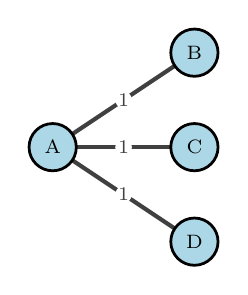
\begin{tikzpicture}[scale = 0.6]
    \Vertex [IdAsLabel, y=1] {A} \Vertex[IdAsLabel,x=3,y=3]{B} \Vertex[IdAsLabel, x=3, y =1]{C} \Vertex[IdAsLabel, x=3,y=-1]{D}
    \Edge[label=1](A)(B)
    \Edge[label=1](A)(C)
    \Edge[label=1](A)(D)
    % \draw[red, style=dashed] (0, 0) .. controls (3.5,-4) .. (3.5, 1);
    % \draw[red, style=dashed] (5, 1) .. controls (5,-1) .. (8, -1);
    \end{tikzpicture}
    \hspace{1cm}
    \begin{tikzpicture}[scale = 0.6]
    \node[inner sep=0pt] (russell) at (-0.3,-1)
    {\includegraphics[width=.025\textwidth]{images/scisssors.png}};
    \Vertex [y=1] {A} \Vertex[label=0,x=3,y=-1]{B} \Vertex[label=0, x=3, y =1]{C} \Vertex[label=1, x=3,y=3]{D}
    \Edge[label=1,RGB,color={250,70,15}](A)(B)
    \Edge[label=1,RGB,color={250,70,15}](A)(C)
    \Edge[label=1](A)(D)
    % \draw[red, style=dashed] (0, 0) .. controls (3.5,-4) .. (3.5, 1);
    \draw[red, style=dashed] (0, -1) .. controls (2.98,2.5) .. (3.75, 1.25);
    \end{tikzpicture}
    \caption{The subgraph $H$ is on the left, and the optimal cut of $H$ for the partial assignment $[1,0,0]$ is on the right.}
    \label{FIG:PartialAssignEx}
\end{figure}